\documentclass[]{article}
\usepackage{lmodern}
\usepackage{amssymb,amsmath}
\usepackage{ifxetex,ifluatex}
\usepackage{fixltx2e} % provides \textsubscript
\ifnum 0\ifxetex 1\fi\ifluatex 1\fi=0 % if pdftex
  \usepackage[T1]{fontenc}
  \usepackage[utf8]{inputenc}
\else % if luatex or xelatex
  \ifxetex
    \usepackage{mathspec}
  \else
    \usepackage{fontspec}
  \fi
  \defaultfontfeatures{Ligatures=TeX,Scale=MatchLowercase}
\fi
% use upquote if available, for straight quotes in verbatim environments
\IfFileExists{upquote.sty}{\usepackage{upquote}}{}
% use microtype if available
\IfFileExists{microtype.sty}{%
\usepackage{microtype}
\UseMicrotypeSet[protrusion]{basicmath} % disable protrusion for tt fonts
}{}
\usepackage[margin=1in]{geometry}
\usepackage{hyperref}
\hypersetup{unicode=true,
            pdftitle={Final Project - SDS II},
            pdfborder={0 0 0},
            breaklinks=true}
\urlstyle{same}  % don't use monospace font for urls
\usepackage{color}
\usepackage{fancyvrb}
\newcommand{\VerbBar}{|}
\newcommand{\VERB}{\Verb[commandchars=\\\{\}]}
\DefineVerbatimEnvironment{Highlighting}{Verbatim}{commandchars=\\\{\}}
% Add ',fontsize=\small' for more characters per line
\usepackage{framed}
\definecolor{shadecolor}{RGB}{248,248,248}
\newenvironment{Shaded}{\begin{snugshade}}{\end{snugshade}}
\newcommand{\AlertTok}[1]{\textcolor[rgb]{0.94,0.16,0.16}{#1}}
\newcommand{\AnnotationTok}[1]{\textcolor[rgb]{0.56,0.35,0.01}{\textbf{\textit{#1}}}}
\newcommand{\AttributeTok}[1]{\textcolor[rgb]{0.77,0.63,0.00}{#1}}
\newcommand{\BaseNTok}[1]{\textcolor[rgb]{0.00,0.00,0.81}{#1}}
\newcommand{\BuiltInTok}[1]{#1}
\newcommand{\CharTok}[1]{\textcolor[rgb]{0.31,0.60,0.02}{#1}}
\newcommand{\CommentTok}[1]{\textcolor[rgb]{0.56,0.35,0.01}{\textit{#1}}}
\newcommand{\CommentVarTok}[1]{\textcolor[rgb]{0.56,0.35,0.01}{\textbf{\textit{#1}}}}
\newcommand{\ConstantTok}[1]{\textcolor[rgb]{0.00,0.00,0.00}{#1}}
\newcommand{\ControlFlowTok}[1]{\textcolor[rgb]{0.13,0.29,0.53}{\textbf{#1}}}
\newcommand{\DataTypeTok}[1]{\textcolor[rgb]{0.13,0.29,0.53}{#1}}
\newcommand{\DecValTok}[1]{\textcolor[rgb]{0.00,0.00,0.81}{#1}}
\newcommand{\DocumentationTok}[1]{\textcolor[rgb]{0.56,0.35,0.01}{\textbf{\textit{#1}}}}
\newcommand{\ErrorTok}[1]{\textcolor[rgb]{0.64,0.00,0.00}{\textbf{#1}}}
\newcommand{\ExtensionTok}[1]{#1}
\newcommand{\FloatTok}[1]{\textcolor[rgb]{0.00,0.00,0.81}{#1}}
\newcommand{\FunctionTok}[1]{\textcolor[rgb]{0.00,0.00,0.00}{#1}}
\newcommand{\ImportTok}[1]{#1}
\newcommand{\InformationTok}[1]{\textcolor[rgb]{0.56,0.35,0.01}{\textbf{\textit{#1}}}}
\newcommand{\KeywordTok}[1]{\textcolor[rgb]{0.13,0.29,0.53}{\textbf{#1}}}
\newcommand{\NormalTok}[1]{#1}
\newcommand{\OperatorTok}[1]{\textcolor[rgb]{0.81,0.36,0.00}{\textbf{#1}}}
\newcommand{\OtherTok}[1]{\textcolor[rgb]{0.56,0.35,0.01}{#1}}
\newcommand{\PreprocessorTok}[1]{\textcolor[rgb]{0.56,0.35,0.01}{\textit{#1}}}
\newcommand{\RegionMarkerTok}[1]{#1}
\newcommand{\SpecialCharTok}[1]{\textcolor[rgb]{0.00,0.00,0.00}{#1}}
\newcommand{\SpecialStringTok}[1]{\textcolor[rgb]{0.31,0.60,0.02}{#1}}
\newcommand{\StringTok}[1]{\textcolor[rgb]{0.31,0.60,0.02}{#1}}
\newcommand{\VariableTok}[1]{\textcolor[rgb]{0.00,0.00,0.00}{#1}}
\newcommand{\VerbatimStringTok}[1]{\textcolor[rgb]{0.31,0.60,0.02}{#1}}
\newcommand{\WarningTok}[1]{\textcolor[rgb]{0.56,0.35,0.01}{\textbf{\textit{#1}}}}
\usepackage{graphicx,grffile}
\makeatletter
\def\maxwidth{\ifdim\Gin@nat@width>\linewidth\linewidth\else\Gin@nat@width\fi}
\def\maxheight{\ifdim\Gin@nat@height>\textheight\textheight\else\Gin@nat@height\fi}
\makeatother
% Scale images if necessary, so that they will not overflow the page
% margins by default, and it is still possible to overwrite the defaults
% using explicit options in \includegraphics[width, height, ...]{}
\setkeys{Gin}{width=\maxwidth,height=\maxheight,keepaspectratio}
\IfFileExists{parskip.sty}{%
\usepackage{parskip}
}{% else
\setlength{\parindent}{0pt}
\setlength{\parskip}{6pt plus 2pt minus 1pt}
}
\setlength{\emergencystretch}{3em}  % prevent overfull lines
\providecommand{\tightlist}{%
  \setlength{\itemsep}{0pt}\setlength{\parskip}{0pt}}
\setcounter{secnumdepth}{0}
% Redefines (sub)paragraphs to behave more like sections
\ifx\paragraph\undefined\else
\let\oldparagraph\paragraph
\renewcommand{\paragraph}[1]{\oldparagraph{#1}\mbox{}}
\fi
\ifx\subparagraph\undefined\else
\let\oldsubparagraph\subparagraph
\renewcommand{\subparagraph}[1]{\oldsubparagraph{#1}\mbox{}}
\fi

%%% Use protect on footnotes to avoid problems with footnotes in titles
\let\rmarkdownfootnote\footnote%
\def\footnote{\protect\rmarkdownfootnote}

%%% Change title format to be more compact
\usepackage{titling}

% Create subtitle command for use in maketitle
\providecommand{\subtitle}[1]{
  \posttitle{
    \begin{center}\large#1\end{center}
    }
}

\setlength{\droptitle}{-2em}

  \title{Final Project - SDS II}
    \pretitle{\vspace{\droptitle}\centering\huge}
  \posttitle{\par}
    \author{Fabio Montello}
    \preauthor{\centering\large\emph}
  \postauthor{\par}
      \predate{\centering\large\emph}
  \postdate{\par}
    \date{05/08/2019}

\usepackage{booktabs}
\usepackage{longtable}
\usepackage{array}
\usepackage{multirow}
\usepackage{wrapfig}
\usepackage{float}
\usepackage{colortbl}
\usepackage{pdflscape}
\usepackage{tabu}
\usepackage{threeparttable}
\usepackage{threeparttablex}
\usepackage[normalem]{ulem}
\usepackage{makecell}
\usepackage{xcolor}

\usepackage{graphicx}

\begin{document}
\maketitle

This work is a full Bayesian analysis, over data regarding the death of
beetles after exposure of different concentration of carbondisulphide.
The aim of this work is to figure out which of the three proposed models
is the best for the given data.

\hypertarget{beetles-data}{%
\section{Beetles data}\label{beetles-data}}

The binary dose-response data used in this work is the one published by
Bliss (1935) and analyzed by Dobson (1983) and represent the number of
beetles killed after 5 hours exposure to carbon disulphide at \(N = 8\)
different concentrations.

Let's have a look at the database:

\begin{Shaded}
\begin{Highlighting}[]
\NormalTok{data =}\StringTok{ }\KeywordTok{list}\NormalTok{( }\DataTypeTok{x =} \KeywordTok{c}\NormalTok{(}\FloatTok{1.6907}\NormalTok{, }\FloatTok{1.7242}\NormalTok{, }\FloatTok{1.7552}\NormalTok{, }\FloatTok{1.7842}\NormalTok{, }\FloatTok{1.8113}\NormalTok{, }\FloatTok{1.8369}\NormalTok{, }\FloatTok{1.8610}\NormalTok{, }\FloatTok{1.8839}\NormalTok{),}
             \DataTypeTok{n =} \KeywordTok{c}\NormalTok{(}\DecValTok{59}\NormalTok{, }\DecValTok{60}\NormalTok{, }\DecValTok{62}\NormalTok{, }\DecValTok{56}\NormalTok{, }\DecValTok{63}\NormalTok{, }\DecValTok{59}\NormalTok{, }\DecValTok{62}\NormalTok{, }\DecValTok{60}\NormalTok{),}
             \DataTypeTok{r =} \KeywordTok{c}\NormalTok{(}\DecValTok{6}\NormalTok{, }\DecValTok{13}\NormalTok{, }\DecValTok{18}\NormalTok{, }\DecValTok{28}\NormalTok{, }\DecValTok{52}\NormalTok{, }\DecValTok{53}\NormalTok{, }\DecValTok{61}\NormalTok{, }\DecValTok{60}\NormalTok{), }
             \DataTypeTok{N =} \DecValTok{8}\NormalTok{)}

\NormalTok{df =}\StringTok{ }\KeywordTok{as.data.frame}\NormalTok{(}\KeywordTok{list}\NormalTok{(}\StringTok{"Concentration"}\NormalTok{ =}\StringTok{ }\NormalTok{data}\OperatorTok{$}\NormalTok{x, }
                        \StringTok{"Number_of_beetles"}\NormalTok{ =}\StringTok{ }\NormalTok{data}\OperatorTok{$}\NormalTok{n, }
                        \StringTok{"Number_killed"}\NormalTok{ =}\StringTok{ }\NormalTok{data}\OperatorTok{$}\NormalTok{r))}

\NormalTok{df}\OperatorTok{$}\NormalTok{Rate =}\StringTok{ }\NormalTok{df}\OperatorTok{$}\NormalTok{Number_killed}\OperatorTok{/}\NormalTok{df}\OperatorTok{$}\NormalTok{Number_of_beetles}
\NormalTok{toprint =}\StringTok{ }\NormalTok{df}
\KeywordTok{names}\NormalTok{(toprint) =}\StringTok{ }\KeywordTok{list}\NormalTok{(}\StringTok{"Concentration"}\NormalTok{, }\StringTok{"Number of beetles"}\NormalTok{, }\StringTok{"Number of dead beetles"}\NormalTok{, }\StringTok{"Death rate"}\NormalTok{)}
\KeywordTok{kable}\NormalTok{(toprint, }\StringTok{"latex"}\NormalTok{, }\DataTypeTok{booktabs =}\NormalTok{ T) }\OperatorTok
\StringTok{  }\KeywordTok{kable_styling}\NormalTok{(}\DataTypeTok{latex_options =} \KeywordTok{c}\NormalTok{(}\StringTok{"striped"}\NormalTok{, }\StringTok{"hold_position"}\NormalTok{))}
\end{Highlighting}
\end{Shaded}

\begin{table}[!h]
\centering
\begin{tabular}{rrrr}
\toprule
Concentration & Number of beetles & Number of dead beetles & Death rate\\
\midrule
\rowcolor{gray!6}  1.6907 & 59 & 6 & 0.1016949\\
1.7242 & 60 & 13 & 0.2166667\\
\rowcolor{gray!6}  1.7552 & 62 & 18 & 0.2903226\\
1.7842 & 56 & 28 & 0.5000000\\
\rowcolor{gray!6}  1.8113 & 63 & 52 & 0.8253968\\
\addlinespace
1.8369 & 59 & 53 & 0.8983051\\
\rowcolor{gray!6}  1.8610 & 62 & 61 & 0.9838710\\
1.8839 & 60 & 60 & 1.0000000\\
\bottomrule
\end{tabular}
\end{table}

Assuming that the observed number of deaths \(r_i\) at each
concentration \(x_i\) is binomial with sample size \(n_i\) and true rate
\(p_i\), we can plot the death rate of our sample:

\begin{Shaded}
\begin{Highlighting}[]
\KeywordTok{plot}\NormalTok{(}\DataTypeTok{x =}\NormalTok{ data}\OperatorTok{$}\NormalTok{x, }\DataTypeTok{y =}\NormalTok{ (data}\OperatorTok{$}\NormalTok{r}\OperatorTok{/}\NormalTok{data}\OperatorTok{$}\NormalTok{n), }
     \DataTypeTok{main =} \StringTok{"Beetles death rate at different concentrations of carbon disulphide"}\NormalTok{,}
     \DataTypeTok{xlab =} \StringTok{"Concentration of carbon disulphide"}\NormalTok{, }
     \DataTypeTok{ylab =} \StringTok{"Beetles death rate"}\NormalTok{,}
     \DataTypeTok{pch =} \DecValTok{16}\NormalTok{, }\DataTypeTok{col =} \StringTok{"royalblue2"}\NormalTok{)}
\end{Highlighting}
\end{Shaded}

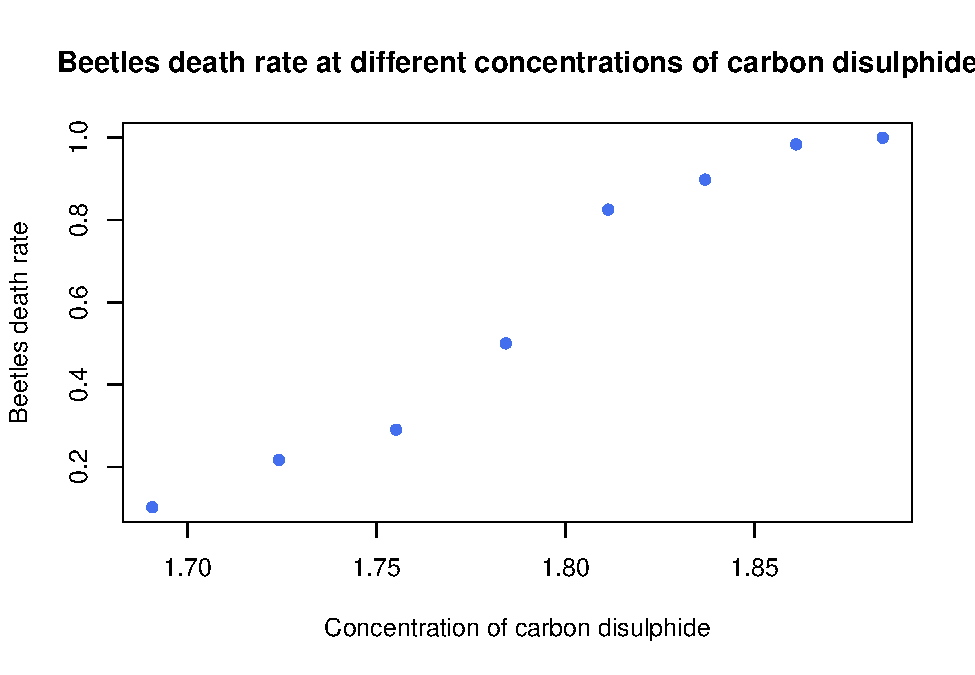
\includegraphics{FinalProject-SDSII_files/figure-latex/unnamed-chunk-2-1.pdf}
We can have a little recap for the feautures of our data:

\begin{itemize}
\tightlist
\item
  \(r_i\) = number of dead beetles \(\in \mathbb{N}^+\)
\item
  \(x_i\) = concentration of carboon disulphide \(\in \mathbb{R}^+\)
\item
  \(n_i\) = sample size \(\in \mathbb{N}^+\)
\item
  \(p_i\) = true death rate \(\in[0,1]\)
\end{itemize}

\hypertarget{models-and-parameters}{%
\section{Models and parameters}\label{models-and-parameters}}

As said previously, we assume that the observed number of deaths \(r_i\)
at each concentration \(x_i\) is binomial, with a sample size equal to
the number of beetles \(n_i\) and a true rate of deaths \(p_i\):
\[Y_i \sim Binomial(n_i, p_i)\] with the parameters
\(n_i \in \mathbb{N}\) and \(p_i \in [0,1]\).

For this purpose, Dobson in 1983 proposed to model the binary
dose-response of deaths with three different types plausible link
functions for \(p_i\). These three models are the logistic, the probit
and the extreme values (complementary log-log): \begin{eqnarray*}
  p_i &=& \frac{\exp(\alpha + \beta x_i)}{1 + \exp(\alpha + \beta x_i)}\\
  p_i &=& \Phi(\alpha + \beta x_i) = \frac{1}{\sqrt{2\pi}}\int _{-\infty }^{\alpha + \beta x_i}e^{-\frac{1}{2}}dt\\
  p_i &=& 1 - \exp(- \exp(\alpha + \beta x_i))
\end{eqnarray*}

Since we have three different models that seems suitable for our data,
we want to do a MCMC simulation with each of these models, and then use
these simulation to compare the models, so to observe which one fits the
data the best.

The models parameters are \(\alpha\) and \(\beta\). In this case we
assume that these parameters are normally distribuited:
\begin{eqnarray*}
  \alpha &\sim& Norm(0,\sigma^{2}_{\alpha})\\
  \beta &\sim& Norm(0,\sigma^{2}_{\beta})
\end{eqnarray*}

We are looking for a non-informative prior choice for these parameters,
so we are going to set for both a \(\sigma^2\) value close to \(\infty\)
or better a low \(\tau = \frac{1}{\sigma^2}\):

\begin{Shaded}
\begin{Highlighting}[]
\NormalTok{  tau_alpha =}\StringTok{ }\NormalTok{tau_beta =}\StringTok{ }\FloatTok{0.00001}
\end{Highlighting}
\end{Shaded}

\hypertarget{likelihood-and-posterior}{%
\section{Likelihood and posterior}\label{likelihood-and-posterior}}

As we know, according to the Bayes theorem, the posterior distribution
can be written as:
\[f(\alpha,\beta | n, r, X) = \frac{f(r | \alpha,\beta, n, X) f(p)}{ f(r)} \propto f(r | \alpha,\beta, n, X) f(\alpha,\beta) \propto  \mathcal{L}(r, \alpha,\beta, n, X) \pi(\alpha) \pi(\beta)\]
The posterior distribution embodies both prior and observed data
information, which is expressed by the prior distribution \(f(p)\) and
the likelihood:

\[
\begin{aligned} 
  \mathcal{L}(r, \alpha,\beta,n, X) &= \prod_{i = 1}^{m}{\displaystyle {\binom {n_i}{r_i}} \; link_f(\alpha,\beta, x_i)^{r_i}\;(1-link_f(\alpha,\beta, x_i))^{n_i-r_i}}\\
                        &\propto \prod_{i = 1}^{m}{ link_f(\alpha,\beta, x_i)^{r_i}\;(1-link_f(\alpha,\beta, x_i))^{n_i-r_i}}\\
\end{aligned}
\] where \(link_f(\alpha,\beta, x_i)\) is either the logistic, the
probit or the extreme values function, according to which link function
we want to use in our model. So we have that our posterior probability
will be: \[
\begin{aligned} 
  f(\alpha,\beta | n, r, X) &\propto \mathcal{L}(r | n, X, \alpha, \beta) \; \pi(\alpha) \: \pi(\beta)\\
                  &\propto \prod_{i = 1}^{m}{ link_f(\alpha,\beta, x_i)^{r_i}\;(1-link_f(\alpha,\beta, x_i))^{n_i-r_i}} \; \frac{1}{\sqrt{2\pi\sigma_{\alpha}^{2}}} e^{-\frac{\alpha^2}{2\sigma_{\alpha}^{2}}} \: \frac{1}{\sqrt{2\pi\sigma_{\beta}^{2}}} e^{-\frac{\beta^2}{2\sigma_{\beta}^{2}}}\\
\end{aligned} 
\]

\hypertarget{bayesian-analysis-with-mcmc}{%
\section{Bayesian Analysis with
MCMC}\label{bayesian-analysis-with-mcmc}}

Before starting any type of analysis, is a good practice to create a
list that contains all the data needed to be processed later on:

\begin{Shaded}
\begin{Highlighting}[]
\NormalTok{data.list=}\StringTok{ }\KeywordTok{list}\NormalTok{(}\DataTypeTok{r =}\NormalTok{ data}\OperatorTok{$}\NormalTok{r,}
                \DataTypeTok{n =}\NormalTok{ data}\OperatorTok{$}\NormalTok{n,}
                \DataTypeTok{x =}\NormalTok{ data}\OperatorTok{$}\NormalTok{x,}
                \DataTypeTok{tau_alpha =}\NormalTok{ tau_alpha,}
                \DataTypeTok{tau_beta =}\NormalTok{ tau_beta,}
                \DataTypeTok{N =} \DecValTok{8}\NormalTok{)}
\end{Highlighting}
\end{Shaded}

It is important also to point out that we are going to standardize each
dose of \(x_i\) about the mean: this gives approximately uncorrelated
regression coefficients, and greatly improves convergence. Of course
this imply that then \(\alpha\) is going to be a latent variable, which
can be derived from \(\alpha^*\) in the model or after the model has
run, simply by inverting the standardization:
\[\alpha = \alpha^* - \beta \bar{x}\] Concerning the constant parameter
\(\alpha^*\), its interpretation corresponds to the expected value of
the response variable \(Y\) when the observed values of all covariates
are equal to zero. Frequently such combination lies outside the range of
the observed covariate values. In such cases, the interpretation of
\(\alpha^*\) is not reliable. Frequently,direct interpretation of
\(\alpha^*\) does not lead to realistic and sensible interpretation. An
alternative is to center around zero all explanatory variables \(X\), by
subtracting their sample mean.

\hypertarget{logistic-model}{%
\subsection{Logistic model}\label{logistic-model}}

As first model for our Bayesian analysis we want to start with the
logistic model: \[ Y_i \sim Binomial(n_i, p_i)\]
\[p_i = \frac{\exp(\alpha + \beta x_i)}{1 + \exp(\alpha + \beta x_i)}\]

All the models presented will be executed through JAGS.\\
As premised previously, the prior distributions for the two parameters
to estimate have been chosen to be uninformative priors, due to our
ignorance over the topic. This means we picked Normal distributions with
mean equal to zero and precision equal to 0.00001 (infinite variance).

Then we can proceed by translating into code the model we formulized
previously, taking into account the link function chosen:

\begin{Shaded}
\begin{Highlighting}[]
\NormalTok{model_}\DecValTok{1}\NormalTok{ =}\StringTok{ "}
\StringTok{      model \{}
\StringTok{       for( i in 1 : N ) \{}
\StringTok{          r[i] ~ dbin(p[i],n[i])}
\StringTok{          logit(p[i]) <- alpha.star + beta * (x[i] - mean(x[]))}
\StringTok{          rhat[i] <- n[i] * p[i]}
\StringTok{       \}}
\StringTok{       alpha = alpha.star - beta * mean(x[])}
\StringTok{       beta ~ dnorm(0.0,tau_beta)}
\StringTok{       alpha.star ~ dnorm(0.0,tau_alpha)   }
\StringTok{    \}"}\NormalTok{;}
\end{Highlighting}
\end{Shaded}

The chains will have different initial values, because this is a good
check for the stationarity of the chain: in fact, a stationary chain is
not influenced by the initial state, hence any different simulation of
the chain should return the same results. The initial values are then
chosen different from each others, but with no particular meaning:

\begin{Shaded}
\begin{Highlighting}[]
\NormalTok{init.list.nod =}\KeywordTok{list}\NormalTok{(}\KeywordTok{list}\NormalTok{(}\DataTypeTok{alpha.star =} \DecValTok{0}\NormalTok{, }\DataTypeTok{beta =}\DecValTok{0}\NormalTok{),}
                    \KeywordTok{list}\NormalTok{(}\DataTypeTok{alpha.star =} \DecValTok{1}\NormalTok{, }\DataTypeTok{beta =}\DecValTok{2}\NormalTok{),}
                    \KeywordTok{list}\NormalTok{(}\DataTypeTok{alpha.star =} \DecValTok{3}\NormalTok{, }\DataTypeTok{beta =}\DecValTok{0}\NormalTok{))}
\end{Highlighting}
\end{Shaded}

In order to get more accurate results, the model will run 3 different
chains, where the number of replications for each one it's equal to
11000. From each one the first 1000 observation have been burnt, just to
remove the initial noise of the first states of the chains, and to take
just the part where we wish the chains become stationary.

\begin{Shaded}
\begin{Highlighting}[]
\NormalTok{mcmc_res =}\StringTok{ }\KeywordTok{jags}\NormalTok{( }\DataTypeTok{model.file =} \KeywordTok{textConnection}\NormalTok{(model_}\DecValTok{1}\NormalTok{),}
                  \DataTypeTok{data =}\NormalTok{ data.list, }
                  \DataTypeTok{n.chains =} \DecValTok{3}\NormalTok{, }
                  \DataTypeTok{n.iter =} \DecValTok{11000}\NormalTok{, }
                  \DataTypeTok{n.burnin =} \DecValTok{1000}\NormalTok{,}
                  \DataTypeTok{inits =}\NormalTok{ init.list.nod, }
                  \DataTypeTok{parameters.to.save =} \KeywordTok{c}\NormalTok{(}\StringTok{"alpha"}\NormalTok{,}\StringTok{"alpha.star"}\NormalTok{,}\StringTok{"beta"}\NormalTok{, }\StringTok{"rhat"}\NormalTok{))}
\end{Highlighting}
\end{Shaded}

\begin{verbatim}
## module glm loaded
\end{verbatim}

\begin{verbatim}
## Compiling model graph
##    Resolving undeclared variables
##    Allocating nodes
## Graph information:
##    Observed stochastic nodes: 8
##    Unobserved stochastic nodes: 2
##    Total graph size: 74
## 
## Initializing model
\end{verbatim}

After the model has been fitted and compiled properly, it's time to have
a look at a first summary of the results:

\begin{Shaded}
\begin{Highlighting}[]
\NormalTok{logit_res <-}\StringTok{ }\NormalTok{mcmc_res}
\KeywordTok{print}\NormalTok{(mcmc_res)}
\end{Highlighting}
\end{Shaded}

\begin{verbatim}
## Inference for Bugs model at "5", fit using jags,
##  3 chains, each with 11000 iterations (first 1000 discarded), n.thin = 10
##  n.sims = 3000 iterations saved
##            mu.vect sd.vect    2.5%     25%     50%     75%   97.5%  Rhat
## alpha      -61.199   5.644 -72.062 -64.874 -60.990 -57.538 -51.312 1.002
## alpha.star   0.751   0.146   0.471   0.660   0.749   0.842   1.025 1.004
## beta        34.543   3.167  28.989  32.484  34.423  36.604  40.600 1.005
## rhat[1]      3.537   1.494   1.912   2.819   3.409   4.075   5.663 1.003
## rhat[2]      9.878   1.998   6.689   8.672   9.759  10.953  13.410 1.003
## rhat[3]     22.449   2.261  18.306  21.010  22.426  23.869  26.756 1.002
## rhat[4]     33.933   1.823  30.184  32.779  33.944  35.113  37.303 1.002
## rhat[5]     50.135   1.726  46.590  49.057  50.206  51.289  53.297 1.003
## rhat[6]     53.284   1.204  50.815  52.575  53.366  54.097  55.289 1.011
## rhat[7]     59.188   0.883  57.470  58.747  59.276  59.735  60.452 1.042
## rhat[8]     58.704   0.619  57.705  58.468  58.772  59.027  59.392 1.103
## deviance    39.878  13.189  37.482  38.010  38.822  40.345  45.510 1.028
##            n.eff
## alpha       2100
## alpha.star  1700
## beta        2200
## rhat[1]     1300
## rhat[2]     1200
## rhat[3]     1100
## rhat[4]     1600
## rhat[5]     2600
## rhat[6]     2700
## rhat[7]     2500
## rhat[8]     2700
## deviance    1900
## 
## For each parameter, n.eff is a crude measure of effective sample size,
## and Rhat is the potential scale reduction factor (at convergence, Rhat=1).
## 
## DIC info (using the rule, pD = var(deviance)/2)
## pD = 87.0 and DIC = 126.9
## DIC is an estimate of expected predictive error (lower deviance is better).
\end{verbatim}

Before discussing any kind of conclusion on the results is good practice
to check if the model is proper, which mean that the distribution
converged.\\
A first indicator of convergence can be checked in the summary printed
above: the \(\hat{R}\) is a test that checks the convergence of a serie,
and it is equal to 1 when the series converges. As we can see, all the
parameters displayed seem to have a value very close to 1, hence we can
start assuming the series are converging.

To go further with the checks, it is possible to have a look also at the
traceplots and the mean plots.

The traceplot helps us check whether a Markov Chain has a random
sampling behavior, and assess mixing across chains and convergence:

\begin{Shaded}
\begin{Highlighting}[]
\NormalTok{chain_print =}\StringTok{ }\KeywordTok{ggs}\NormalTok{(}\KeywordTok{as.mcmc}\NormalTok{(mcmc_res))}
\KeywordTok{ggs_traceplot}\NormalTok{(chain_print)}
\end{Highlighting}
\end{Shaded}

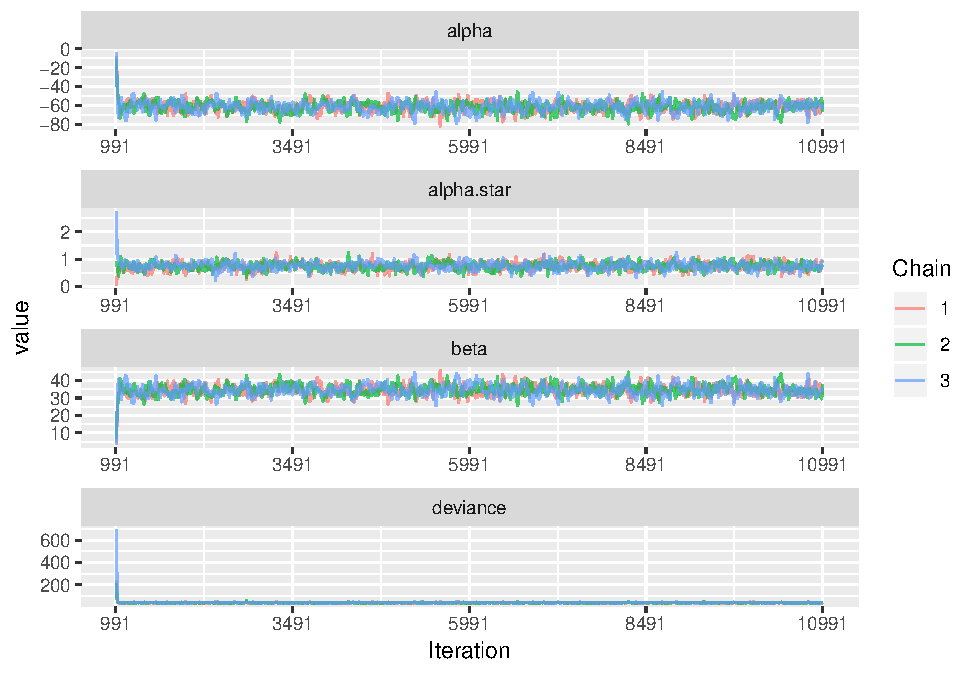
\includegraphics{FinalProject-SDSII_files/figure-latex/unnamed-chunk-9-1.pdf}
The chains for all the parameters does not seem to follow some patterns,
depending on the states or on the initial points. Having a random
behaviour over the same interval of values is a good indicator of the
convergence of the chain.

This can also be confirmed by the running mean plot, which shows how the
mean of the estimator converges to the final average value after a
while:

\begin{Shaded}
\begin{Highlighting}[]
\KeywordTok{ggs_running}\NormalTok{(chain_print)}
\end{Highlighting}
\end{Shaded}

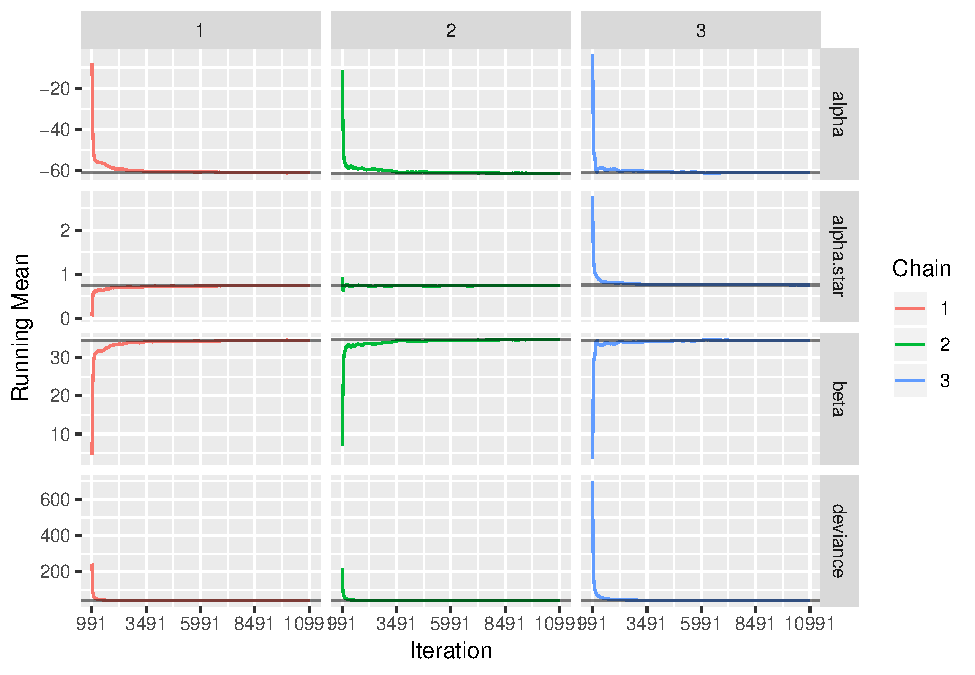
\includegraphics{FinalProject-SDSII_files/figure-latex/unnamed-chunk-10-1.pdf}

Another important check for the presence of pattern in the chain is the
autocorrelation plot, which let us find out if in any part of the chain
there are any some parts that are correlated each other, meaning the
data seems to follow some patterns. What we are expecting is an
autocorrelation plot that has values as close as possible to 0, avoiding
any loop occurance.

\begin{Shaded}
\begin{Highlighting}[]
\KeywordTok{ggs_autocorrelation}\NormalTok{(chain_print, }\DataTypeTok{nLags =} \DecValTok{30}\NormalTok{)}
\end{Highlighting}
\end{Shaded}

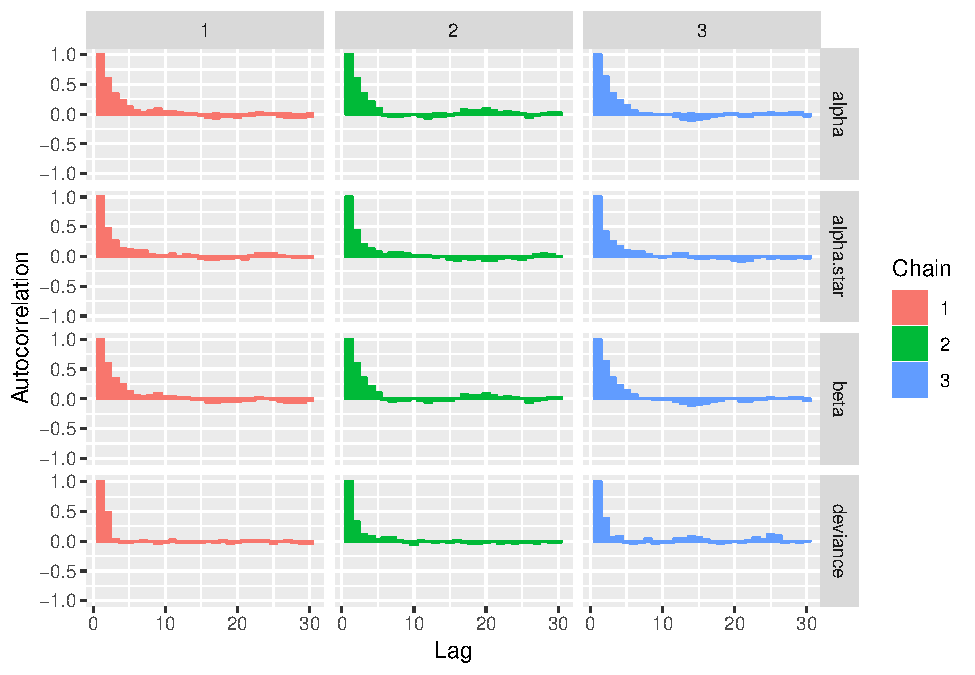
\includegraphics{FinalProject-SDSII_files/figure-latex/unnamed-chunk-11-1.pdf}
As we can see, after an initial state of autocorrelation, this seems to
disappear almost totally by getting very close to zero. These three
results together give us a solid proof of the convergence of our chains.

A final step, and good practice, to assess the convergence is to
estimate the density of the parameters:

\begin{Shaded}
\begin{Highlighting}[]
\KeywordTok{ggs_density}\NormalTok{(chain_print)}
\end{Highlighting}
\end{Shaded}

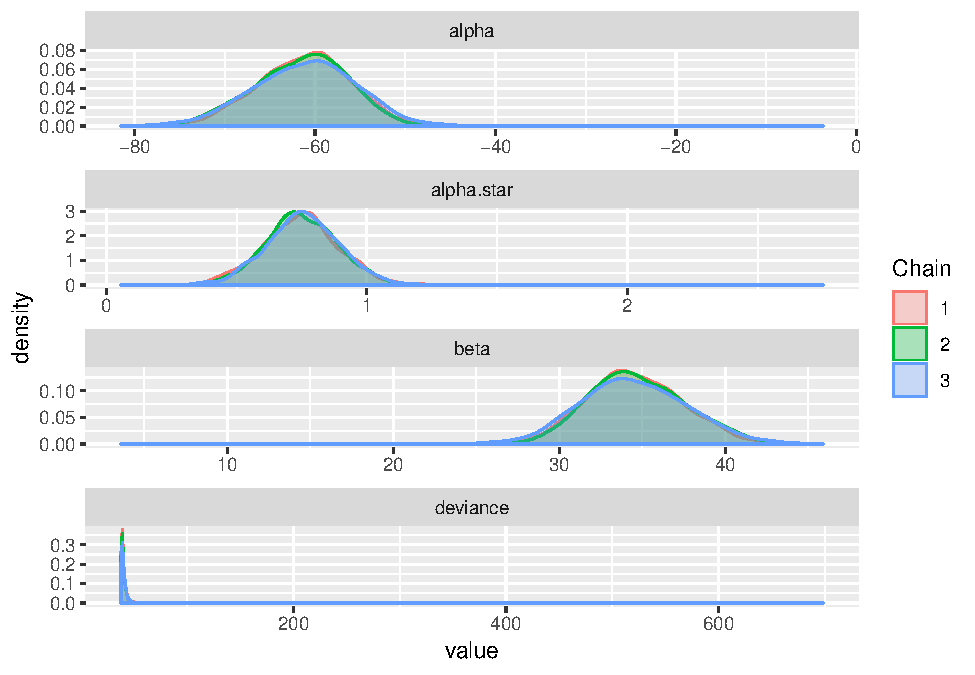
\includegraphics{FinalProject-SDSII_files/figure-latex/unnamed-chunk-12-1.pdf}

The presence of a smooth unimodal distribution is desirable, since it
means that the chains have found the stationarity in the interval around
the mode of the distribution. Here we can see that for the 4 chains,
results are more or less identical, hence it is also another indicator
of the goodness of this model.

Once we made sure the parameters we estimated have been correctly
simulated, we can proceed by visualizing our logistic model with the
data we had:

\begin{Shaded}
\begin{Highlighting}[]
\NormalTok{alpha <-}\KeywordTok{as.numeric}\NormalTok{(mcmc_res}\OperatorTok{$}\NormalTok{BUGSoutput}\OperatorTok{$}\NormalTok{mean}\OperatorTok{$}\NormalTok{alpha) }
\NormalTok{beta <-}\StringTok{ }\KeywordTok{as.numeric}\NormalTok{(mcmc_res}\OperatorTok{$}\NormalTok{BUGSoutput}\OperatorTok{$}\NormalTok{mean}\OperatorTok{$}\NormalTok{beta)}

\NormalTok{logit <-}\StringTok{ }\ControlFlowTok{function}\NormalTok{(x, a, b) }\KeywordTok{return}\NormalTok{(}\KeywordTok{exp}\NormalTok{(a }\OperatorTok{+}\StringTok{ }\NormalTok{b }\OperatorTok{*}\StringTok{ }\NormalTok{x)}\OperatorTok{/}\NormalTok{(}\DecValTok{1}\OperatorTok{+}\KeywordTok{exp}\NormalTok{(a }\OperatorTok{+}\StringTok{ }\NormalTok{b }\OperatorTok{*}\StringTok{ }\NormalTok{x)))}

\KeywordTok{plot}\NormalTok{(}\DataTypeTok{x =}\NormalTok{ data}\OperatorTok{$}\NormalTok{x, }\DataTypeTok{y =}\NormalTok{ (data}\OperatorTok{$}\NormalTok{r}\OperatorTok{/}\NormalTok{data}\OperatorTok{$}\NormalTok{n), }
     \DataTypeTok{main =} \StringTok{"Beetles death rate - Logit model"}\NormalTok{,}
     \DataTypeTok{xlab =} \StringTok{"Concentration of carbon disulphide"}\NormalTok{, }
     \DataTypeTok{ylab =} \StringTok{"Beetles death rate"}\NormalTok{,}
     \DataTypeTok{pch =} \DecValTok{16}\NormalTok{, }\DataTypeTok{col =} \StringTok{"royalblue2"}\NormalTok{)}

\KeywordTok{curve}\NormalTok{(}\KeywordTok{logit}\NormalTok{(x, alpha, beta), }\DataTypeTok{add =}\NormalTok{ T, }\DataTypeTok{col =} \StringTok{'red2'}\NormalTok{, }\DataTypeTok{lwd =} \FloatTok{1.5}\NormalTok{)}
\end{Highlighting}
\end{Shaded}

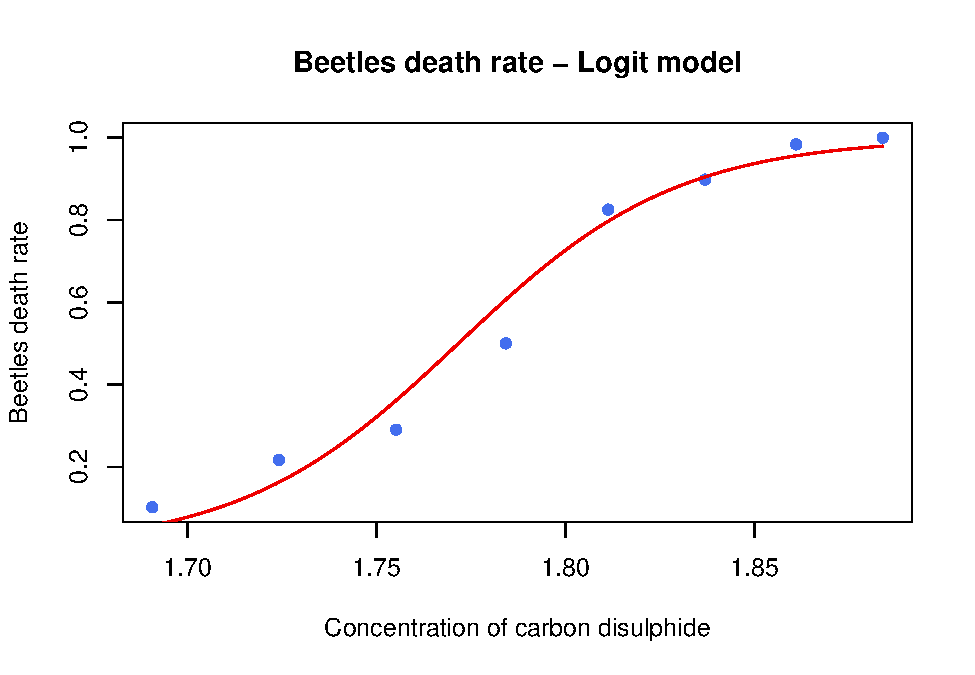
\includegraphics{FinalProject-SDSII_files/figure-latex/unnamed-chunk-13-1.pdf}

The model seems correct and graphically fitting the data. Let's have a
look at the confidence interval values:

\begin{Shaded}
\begin{Highlighting}[]
\KeywordTok{print}\NormalTok{(mcmc_res}\OperatorTok{$}\NormalTok{BUGSoutput}\OperatorTok{$}\NormalTok{summary[}\DecValTok{1}\OperatorTok{:}\DecValTok{4}\NormalTok{, }\KeywordTok{c}\NormalTok{(}\DecValTok{1}\OperatorTok{:}\DecValTok{3}\NormalTok{,}\DecValTok{7}\NormalTok{)])}
\end{Highlighting}
\end{Shaded}

\begin{verbatim}
##                   mean         sd        2.5%      97.5%
## alpha      -61.1986841  5.6438027 -72.0618660 -51.312251
## alpha.star   0.7511321  0.1456266   0.4711782   1.024682
## beta        34.5427416  3.1673761  28.9889496  40.599850
## deviance    39.8778407 13.1890541  37.4820501  45.509700
\end{verbatim}

\begin{Shaded}
\begin{Highlighting}[]
\NormalTok{alpha25 <-}\KeywordTok{as.numeric}\NormalTok{(mcmc_res}\OperatorTok{$}\NormalTok{BUGSoutput}\OperatorTok{$}\NormalTok{summary[}\DecValTok{1}\NormalTok{,}\DecValTok{3}\NormalTok{]) }
\NormalTok{beta25 <-}\StringTok{ }\KeywordTok{as.numeric}\NormalTok{(mcmc_res}\OperatorTok{$}\NormalTok{BUGSoutput}\OperatorTok{$}\NormalTok{summary[}\DecValTok{3}\NormalTok{,}\DecValTok{3}\NormalTok{])}
\NormalTok{alpha975 <-}\KeywordTok{as.numeric}\NormalTok{(mcmc_res}\OperatorTok{$}\NormalTok{BUGSoutput}\OperatorTok{$}\NormalTok{summary[}\DecValTok{1}\NormalTok{,}\DecValTok{7}\NormalTok{]) }
\NormalTok{beta975 <-}\StringTok{ }\KeywordTok{as.numeric}\NormalTok{(mcmc_res}\OperatorTok{$}\NormalTok{BUGSoutput}\OperatorTok{$}\NormalTok{summary[}\DecValTok{3}\NormalTok{,}\DecValTok{7}\NormalTok{])}

\KeywordTok{plot}\NormalTok{(}\DataTypeTok{x =}\NormalTok{ data}\OperatorTok{$}\NormalTok{x, }\DataTypeTok{y =}\NormalTok{ (data}\OperatorTok{$}\NormalTok{r}\OperatorTok{/}\NormalTok{data}\OperatorTok{$}\NormalTok{n), }
     \DataTypeTok{main =} \StringTok{"Beetles death rate - Logit model confidence intervals"}\NormalTok{,}
     \DataTypeTok{xlab =} \StringTok{"Concentration of carbon disulphide"}\NormalTok{, }
     \DataTypeTok{ylab =} \StringTok{"Beetles death rate"}\NormalTok{,}
     \DataTypeTok{pch =} \DecValTok{16}\NormalTok{, }\DataTypeTok{col =} \StringTok{"royalblue2"}\NormalTok{, }\DataTypeTok{xlim =} \KeywordTok{c}\NormalTok{(}\DecValTok{1}\NormalTok{,}\DecValTok{3}\NormalTok{))}

\KeywordTok{curve}\NormalTok{(}\KeywordTok{logit}\NormalTok{(x, alpha, beta), }\DataTypeTok{add =}\NormalTok{ T, }\DataTypeTok{col =} \StringTok{'red2'}\NormalTok{, }\DataTypeTok{lwd =} \FloatTok{1.5}\NormalTok{)}
\KeywordTok{curve}\NormalTok{(}\KeywordTok{logit}\NormalTok{(x, alpha25, beta25), }\DataTypeTok{add =}\NormalTok{ T, }\DataTypeTok{lwd =} \DecValTok{1}\NormalTok{, }\DataTypeTok{lty =} \DecValTok{2}\NormalTok{, }\DataTypeTok{col =} \StringTok{'azure4'}\NormalTok{)}
\KeywordTok{curve}\NormalTok{(}\KeywordTok{logit}\NormalTok{(x, alpha975, beta975), }\DataTypeTok{add =}\NormalTok{ T, }\DataTypeTok{lwd =} \DecValTok{1}\NormalTok{, }\DataTypeTok{lty =} \DecValTok{2}\NormalTok{, }\DataTypeTok{col =} \StringTok{'azure4'}\NormalTok{)}
\end{Highlighting}
\end{Shaded}

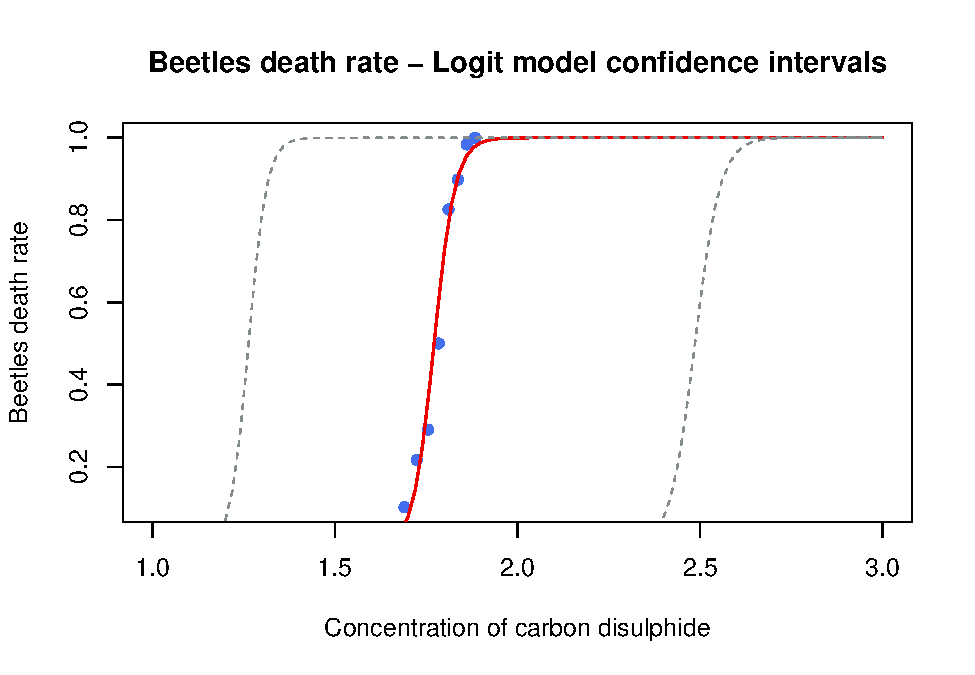
\includegraphics{FinalProject-SDSII_files/figure-latex/unnamed-chunk-15-1.pdf}

\hypertarget{probit-model}{%
\subsection{Probit model}\label{probit-model}}

After the logistic model, the second model we want to work with is the
probit model: \[ Y_i \sim Binomial(n_i, p_i)\]
\[ p_i = \Phi(\alpha + \beta x_i) = \frac{1}{\sqrt{2\pi}}\int _{-\infty }^{\alpha + \beta x_i}e^{-\frac{1}{2}}dt \]

The only variation in respect with the previous model is the link
function, that this time is a probit function. All the settings of the
Markov Chain, the prior distribution, the number of chains, the initial
values, number of iterations, precision value, size of burn-in remained
exactly the same.

\begin{Shaded}
\begin{Highlighting}[]
\NormalTok{model_}\DecValTok{2}\NormalTok{ =}\StringTok{ "}
\StringTok{      model \{}
\StringTok{       for( i in 1 : N ) \{}
\StringTok{          r[i] ~ dbin(p[i],n[i])}
\StringTok{          probit(p[i]) <- alpha.star + beta * (x[i] - mean(x[]))}
\StringTok{          rhat[i] <- n[i] * p[i]}
\StringTok{       \}}
\StringTok{       alpha = alpha.star - beta * mean(x[])}
\StringTok{       beta ~ dnorm(0.0,tau_beta)}
\StringTok{       alpha.star ~ dnorm(0.0,tau_alpha)   }
\StringTok{    \}"}

\NormalTok{init.list.nod =}\KeywordTok{list}\NormalTok{(}\KeywordTok{list}\NormalTok{(}\DataTypeTok{alpha.star =} \DecValTok{0}\NormalTok{, }\DataTypeTok{beta =}\DecValTok{0}\NormalTok{),}
                    \KeywordTok{list}\NormalTok{(}\DataTypeTok{alpha.star =} \DecValTok{1}\NormalTok{, }\DataTypeTok{beta =}\DecValTok{2}\NormalTok{),}
                    \KeywordTok{list}\NormalTok{(}\DataTypeTok{alpha.star =} \DecValTok{3}\NormalTok{, }\DataTypeTok{beta =}\DecValTok{0}\NormalTok{))}

\NormalTok{mcmc_res =}\StringTok{ }\KeywordTok{jags}\NormalTok{( }\DataTypeTok{model.file =} \KeywordTok{textConnection}\NormalTok{(model_}\DecValTok{2}\NormalTok{),}
                  \DataTypeTok{data =}\NormalTok{ data.list, }
                  \DataTypeTok{n.chains =} \DecValTok{3}\NormalTok{, }
                  \DataTypeTok{n.iter =} \DecValTok{11000}\NormalTok{, }
                  \DataTypeTok{n.burnin =} \DecValTok{1000}\NormalTok{,}
                  \DataTypeTok{inits =}\NormalTok{ init.list.nod, }
                  \DataTypeTok{parameters.to.save =} \KeywordTok{c}\NormalTok{(}\StringTok{"alpha"}\NormalTok{,}\StringTok{"alpha.star"}\NormalTok{,}\StringTok{"beta"}\NormalTok{, }\StringTok{"rhat"}\NormalTok{))}
\end{Highlighting}
\end{Shaded}

\begin{verbatim}
## Compiling model graph
##    Resolving undeclared variables
##    Allocating nodes
## Graph information:
##    Observed stochastic nodes: 8
##    Unobserved stochastic nodes: 2
##    Total graph size: 74
## 
## Initializing model
\end{verbatim}

\begin{Shaded}
\begin{Highlighting}[]
\NormalTok{probit_res <-}\StringTok{ }\NormalTok{mcmc_res}
\KeywordTok{print}\NormalTok{(mcmc_res)}
\end{Highlighting}
\end{Shaded}

\begin{verbatim}
## Inference for Bugs model at "6", fit using jags,
##  3 chains, each with 11000 iterations (first 1000 discarded), n.thin = 10
##  n.sims = 3000 iterations saved
##            mu.vect sd.vect    2.5%     25%     50%     75%   97.5%  Rhat
## alpha      -35.170   2.625 -40.410 -36.897 -35.099 -33.408 -30.130 1.001
## alpha.star   0.449   0.078   0.303   0.396   0.448   0.500   0.606 1.001
## beta        19.861   1.476  17.032  18.867  19.823  20.831  22.818 1.001
## rhat[1]      3.408   1.007   1.751   2.701   3.278   4.032   5.618 1.001
## rhat[2]     10.722   1.698   7.566   9.575  10.593  11.841  14.200 1.001
## rhat[3]     23.476   1.923  19.842  22.167  23.409  24.741  27.307 1.001
## rhat[4]     33.855   1.612  30.723  32.796  33.815  34.922  37.125 1.001
## rhat[5]     49.670   1.617  46.412  48.557  49.718  50.773  52.755 1.001
## rhat[6]     53.330   1.141  50.918  52.601  53.388  54.130  55.401 1.001
## rhat[7]     59.638   0.729  57.998  59.216  59.712  60.157  60.833 1.001
## rhat[8]     59.194   0.356  58.339  59.006  59.250  59.450  59.708 1.001
## deviance    38.318   2.051  36.372  36.890  37.693  39.067  43.929 1.001
##            n.eff
## alpha       3000
## alpha.star  3000
## beta        3000
## rhat[1]     3000
## rhat[2]     3000
## rhat[3]     3000
## rhat[4]     3000
## rhat[5]     3000
## rhat[6]     3000
## rhat[7]     3000
## rhat[8]     3000
## deviance    3000
## 
## For each parameter, n.eff is a crude measure of effective sample size,
## and Rhat is the potential scale reduction factor (at convergence, Rhat=1).
## 
## DIC info (using the rule, pD = var(deviance)/2)
## pD = 2.1 and DIC = 40.4
## DIC is an estimate of expected predictive error (lower deviance is better).
\end{verbatim}

Before anything else, let's check again that the chains converges: the
\(\hat{R}\) information is very close to 1, hence it seems we are
dealing with a stationary chain. Let's have further checks with the
traceplots:

\begin{Shaded}
\begin{Highlighting}[]
\NormalTok{chain_print =}\StringTok{ }\KeywordTok{ggs}\NormalTok{(}\KeywordTok{as.mcmc}\NormalTok{(mcmc_res))}
\KeywordTok{ggs_traceplot}\NormalTok{(chain_print)}
\end{Highlighting}
\end{Shaded}

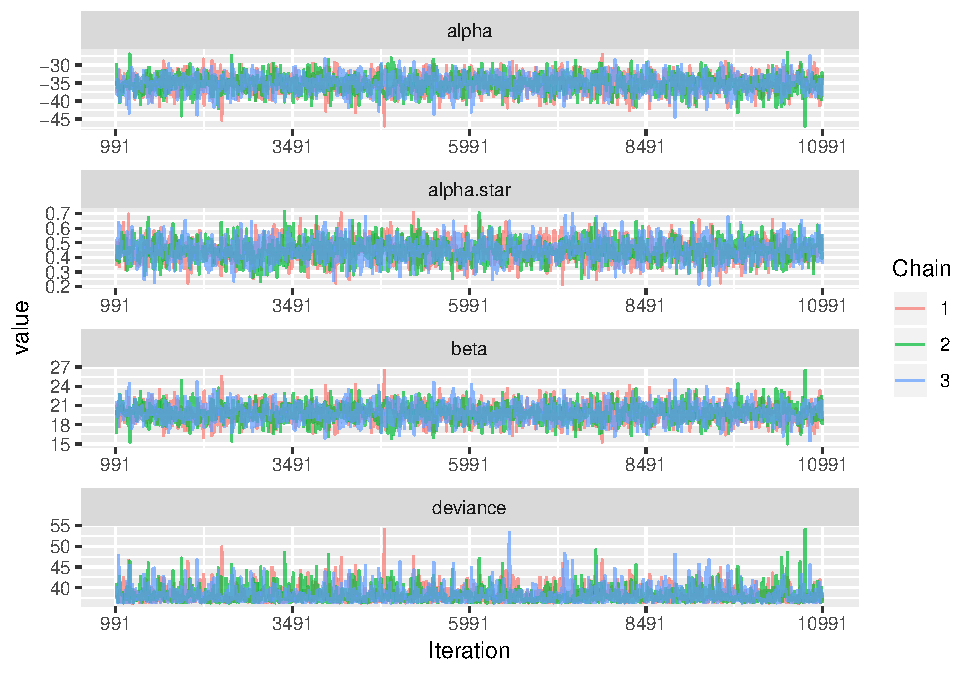
\includegraphics{FinalProject-SDSII_files/figure-latex/unnamed-chunk-17-1.pdf}

The random mixing pattern seems solid, another confermation of the
validity of the chains. We can also have a look at the mean plot:

\begin{Shaded}
\begin{Highlighting}[]
\KeywordTok{ggs_running}\NormalTok{(chain_print)}
\end{Highlighting}
\end{Shaded}

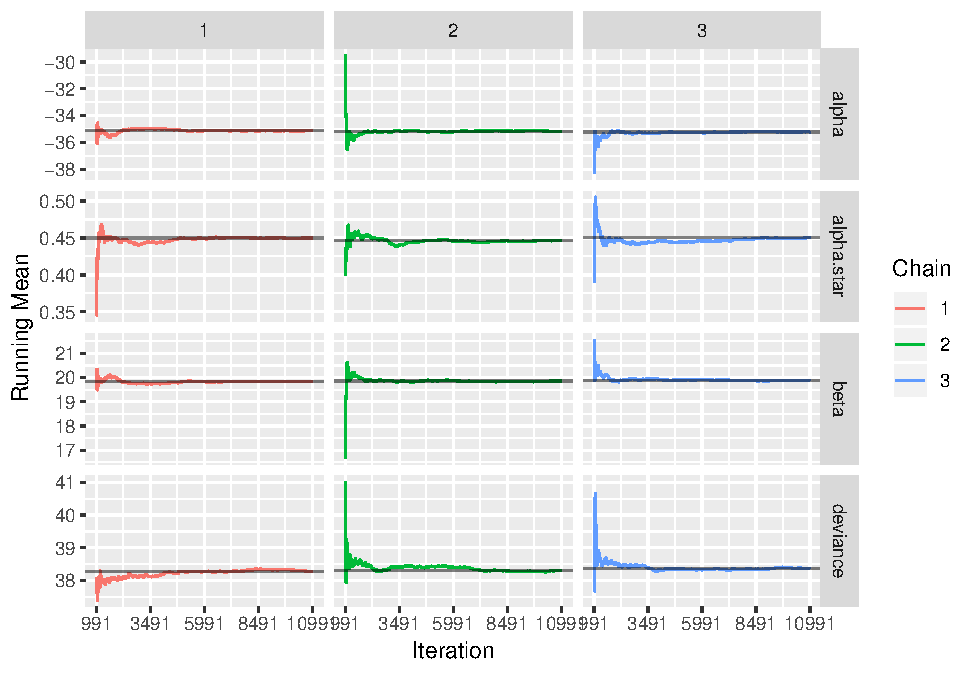
\includegraphics{FinalProject-SDSII_files/figure-latex/unnamed-chunk-18-1.pdf}

which seems to converge properly after few states. Let's check also the
presence of any weird pattern of our chain with the autocorrelation
plot:

\begin{Shaded}
\begin{Highlighting}[]
\KeywordTok{ggs_autocorrelation}\NormalTok{(chain_print, }\DataTypeTok{nLags =} \DecValTok{30}\NormalTok{)}
\end{Highlighting}
\end{Shaded}

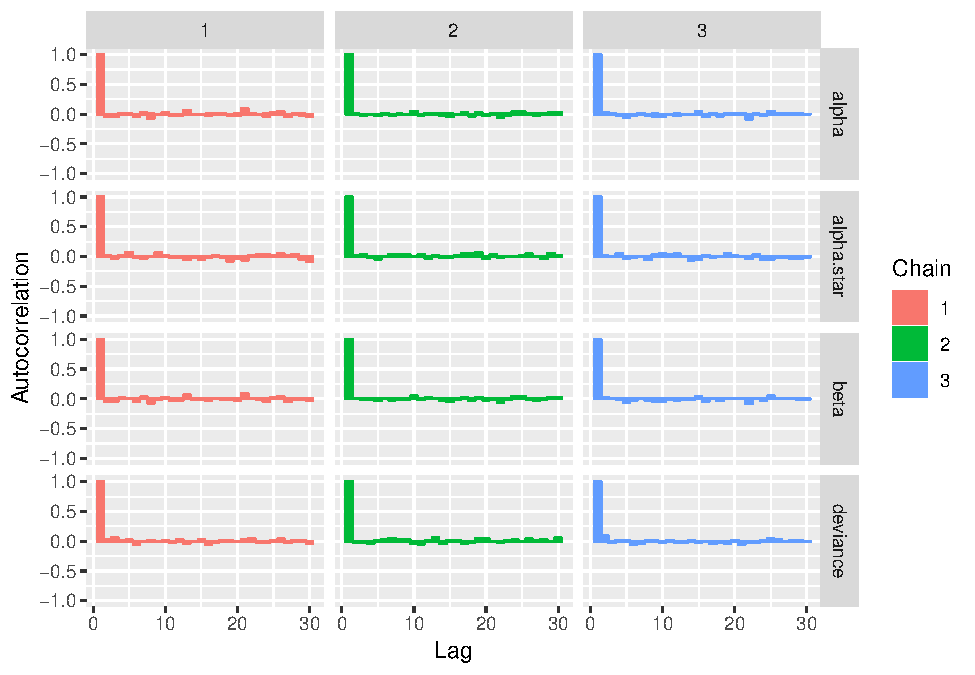
\includegraphics{FinalProject-SDSII_files/figure-latex/unnamed-chunk-19-1.pdf}

where we can observe that, after the initial state, the value is very
close to 0, indicating no correlation at all. Finally, we can also check
the estimated density of the estimators:

\begin{Shaded}
\begin{Highlighting}[]
\KeywordTok{ggs_density}\NormalTok{(chain_print)}
\end{Highlighting}
\end{Shaded}

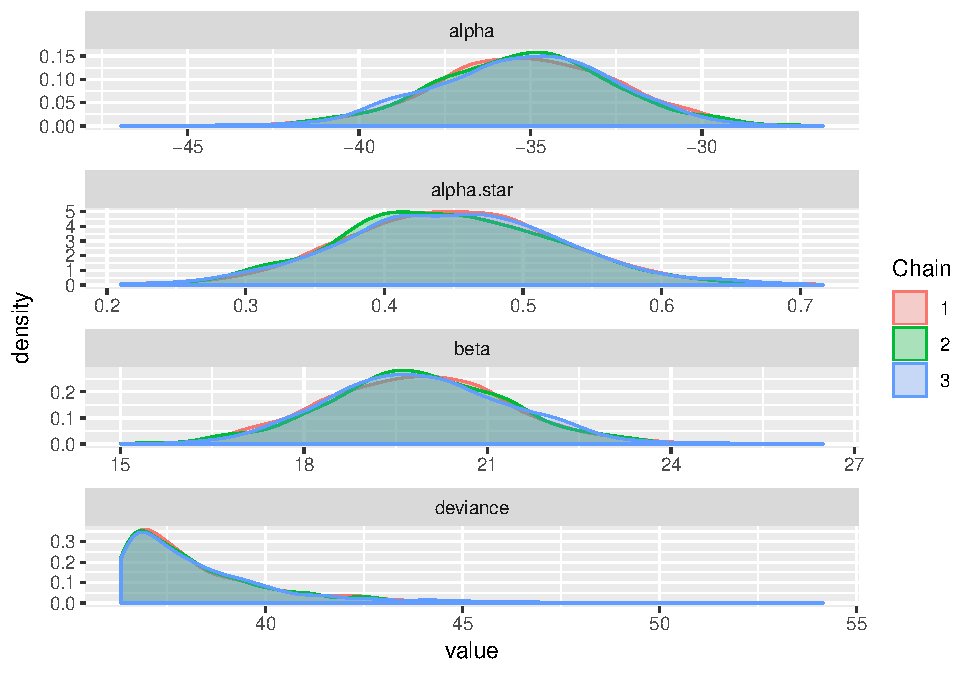
\includegraphics{FinalProject-SDSII_files/figure-latex/unnamed-chunk-20-1.pdf}
Again the distributions seems to be smooth, unimodal and almost
identical between the chains. This is the ultimate assessment of the
stationarity, and thus validity, of the chains in our model.

We can proceed by looking at the goodness of fit of our estimates:

\begin{Shaded}
\begin{Highlighting}[]
\NormalTok{alpha <-}\KeywordTok{as.numeric}\NormalTok{(mcmc_res}\OperatorTok{$}\NormalTok{BUGSoutput}\OperatorTok{$}\NormalTok{mean}\OperatorTok{$}\NormalTok{alpha) }
\NormalTok{beta <-}\StringTok{ }\KeywordTok{as.numeric}\NormalTok{(mcmc_res}\OperatorTok{$}\NormalTok{BUGSoutput}\OperatorTok{$}\NormalTok{mean}\OperatorTok{$}\NormalTok{beta)}

\KeywordTok{plot}\NormalTok{(}\DataTypeTok{x =}\NormalTok{ data}\OperatorTok{$}\NormalTok{x, }\DataTypeTok{y =}\NormalTok{ (data}\OperatorTok{$}\NormalTok{r}\OperatorTok{/}\NormalTok{data}\OperatorTok{$}\NormalTok{n), }
     \DataTypeTok{main =} \StringTok{"Beetles death rate - Probit model"}\NormalTok{,}
     \DataTypeTok{xlab =} \StringTok{"Concentration of carbon disulphide"}\NormalTok{, }
     \DataTypeTok{ylab =} \StringTok{"Beetles death rate"}\NormalTok{,}
     \DataTypeTok{pch =} \DecValTok{16}\NormalTok{, }\DataTypeTok{col =} \StringTok{"royalblue2"}\NormalTok{)}

\KeywordTok{curve}\NormalTok{(}\KeywordTok{pnorm}\NormalTok{(alpha }\OperatorTok{+}\StringTok{ }\NormalTok{(beta }\OperatorTok{*}\StringTok{ }\NormalTok{x), }\DataTypeTok{mean =} \DecValTok{0}\NormalTok{, }\DataTypeTok{sd =} \DecValTok{1}\NormalTok{, }\DataTypeTok{lower.tail =} \OtherTok{TRUE}\NormalTok{), }
      \DataTypeTok{add =}\NormalTok{ T, }\DataTypeTok{col =} \StringTok{'red2'}\NormalTok{, }\DataTypeTok{lwd =} \FloatTok{1.5}\NormalTok{)}
\end{Highlighting}
\end{Shaded}

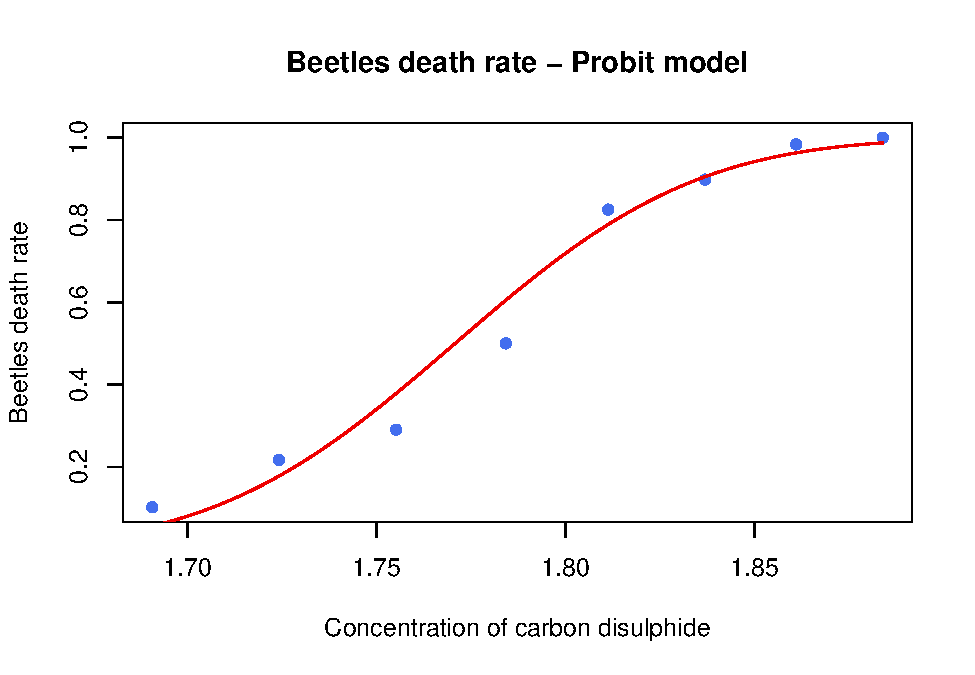
\includegraphics{FinalProject-SDSII_files/figure-latex/unnamed-chunk-21-1.pdf}
Seems to be correct. We can check also the confidence intervals:

\begin{Shaded}
\begin{Highlighting}[]
\KeywordTok{print}\NormalTok{(mcmc_res}\OperatorTok{$}\NormalTok{BUGSoutput}\OperatorTok{$}\NormalTok{summary[}\DecValTok{1}\OperatorTok{:}\DecValTok{4}\NormalTok{, }\KeywordTok{c}\NormalTok{(}\DecValTok{1}\OperatorTok{:}\DecValTok{3}\NormalTok{,}\DecValTok{7}\NormalTok{)])}
\end{Highlighting}
\end{Shaded}

\begin{verbatim}
##                   mean         sd        2.5%       97.5%
## alpha      -35.1702775 2.62529294 -40.4096872 -30.1298130
## alpha.star   0.4491214 0.07790201   0.3027681   0.6062352
## beta        19.8611032 1.47596264  17.0322184  22.8184020
## deviance    38.3183097 2.05135690  36.3720636  43.9291015
\end{verbatim}

\begin{Shaded}
\begin{Highlighting}[]
\NormalTok{alpha25 <-}\KeywordTok{as.numeric}\NormalTok{(mcmc_res}\OperatorTok{$}\NormalTok{BUGSoutput}\OperatorTok{$}\NormalTok{summary[}\DecValTok{1}\NormalTok{,}\DecValTok{3}\NormalTok{]) }
\NormalTok{beta25 <-}\StringTok{ }\KeywordTok{as.numeric}\NormalTok{(mcmc_res}\OperatorTok{$}\NormalTok{BUGSoutput}\OperatorTok{$}\NormalTok{summary[}\DecValTok{3}\NormalTok{,}\DecValTok{3}\NormalTok{])}
\NormalTok{alpha975 <-}\KeywordTok{as.numeric}\NormalTok{(mcmc_res}\OperatorTok{$}\NormalTok{BUGSoutput}\OperatorTok{$}\NormalTok{summary[}\DecValTok{1}\NormalTok{,}\DecValTok{7}\NormalTok{]) }
\NormalTok{beta975 <-}\StringTok{ }\KeywordTok{as.numeric}\NormalTok{(mcmc_res}\OperatorTok{$}\NormalTok{BUGSoutput}\OperatorTok{$}\NormalTok{summary[}\DecValTok{3}\NormalTok{,}\DecValTok{7}\NormalTok{])}

\KeywordTok{plot}\NormalTok{(}\DataTypeTok{x =}\NormalTok{ data}\OperatorTok{$}\NormalTok{x, }\DataTypeTok{y =}\NormalTok{ (data}\OperatorTok{$}\NormalTok{r}\OperatorTok{/}\NormalTok{data}\OperatorTok{$}\NormalTok{n), }
     \DataTypeTok{main =} \StringTok{"Beetles death rate - Probit model confidence intervals"}\NormalTok{,}
     \DataTypeTok{xlab =} \StringTok{"Concentration of carbon disulphide"}\NormalTok{, }
     \DataTypeTok{ylab =} \StringTok{"Beetles death rate"}\NormalTok{,}
     \DataTypeTok{pch =} \DecValTok{16}\NormalTok{, }\DataTypeTok{col =} \StringTok{"royalblue2"}\NormalTok{, }\DataTypeTok{xlim =} \KeywordTok{c}\NormalTok{(}\DecValTok{1}\NormalTok{,}\FloatTok{2.5}\NormalTok{))}

\KeywordTok{curve}\NormalTok{(}\KeywordTok{pnorm}\NormalTok{(alpha }\OperatorTok{+}\StringTok{ }\NormalTok{(beta }\OperatorTok{*}\StringTok{ }\NormalTok{x), }\DataTypeTok{mean =} \DecValTok{0}\NormalTok{, }\DataTypeTok{sd =} \DecValTok{1}\NormalTok{, }\DataTypeTok{lower.tail =} \OtherTok{TRUE}\NormalTok{), }
      \DataTypeTok{add =}\NormalTok{ T, }\DataTypeTok{col =} \StringTok{'red2'}\NormalTok{, }\DataTypeTok{lwd =} \FloatTok{1.5}\NormalTok{)}
\KeywordTok{curve}\NormalTok{(}\KeywordTok{pnorm}\NormalTok{(alpha25 }\OperatorTok{+}\StringTok{ }\NormalTok{(beta25 }\OperatorTok{*}\StringTok{ }\NormalTok{x), }\DataTypeTok{mean =} \DecValTok{0}\NormalTok{, }\DataTypeTok{sd =} \DecValTok{1}\NormalTok{, }\DataTypeTok{lower.tail =} \OtherTok{TRUE}\NormalTok{), }
      \DataTypeTok{add =}\NormalTok{ T, }\DataTypeTok{lwd =} \DecValTok{1}\NormalTok{, }\DataTypeTok{lty =} \DecValTok{2}\NormalTok{, }\DataTypeTok{col =} \StringTok{'azure4'}\NormalTok{)}
\KeywordTok{curve}\NormalTok{(}\KeywordTok{pnorm}\NormalTok{(alpha975 }\OperatorTok{+}\StringTok{ }\NormalTok{(beta975 }\OperatorTok{*}\StringTok{ }\NormalTok{x), }\DataTypeTok{mean =} \DecValTok{0}\NormalTok{, }\DataTypeTok{sd =} \DecValTok{1}\NormalTok{, }\DataTypeTok{lower.tail =} \OtherTok{TRUE}\NormalTok{),}
      \DataTypeTok{add =}\NormalTok{ T, }\DataTypeTok{lwd =} \DecValTok{1}\NormalTok{, }\DataTypeTok{lty =} \DecValTok{2}\NormalTok{, }\DataTypeTok{col =} \StringTok{'azure4'}\NormalTok{)}
\end{Highlighting}
\end{Shaded}

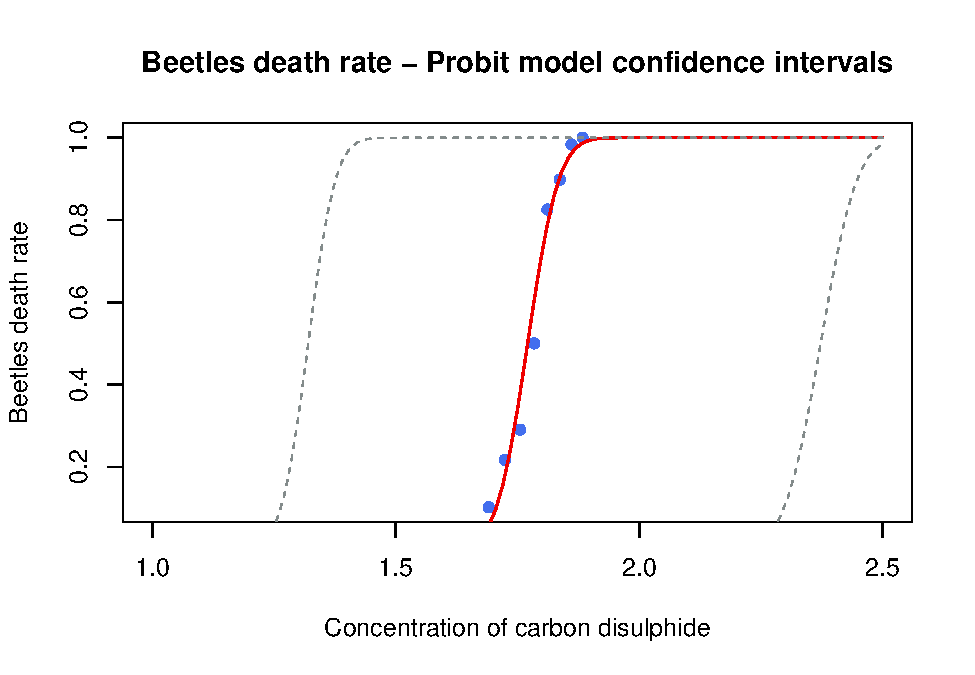
\includegraphics{FinalProject-SDSII_files/figure-latex/unnamed-chunk-23-1.pdf}

\hypertarget{extreme-values-model-or-complementary-log-log-model}{%
\subsection{Extreme values model (or complementary log-log
model)}\label{extreme-values-model-or-complementary-log-log-model}}

Finally, we want to do the same thing for the the extreme values model.
Once again, let's have a look at the model first:
\[ Y_i \sim Binomial(n_i, p_i)\]
\[p_i = 1 - \exp(- \exp(\alpha + \beta x_i))\] For the building of the
model, as previously, we changed only the link function, this time a
extreme values (or complementary log-log) function. Let's have a
reminder on the settings of the Markov Chain: the prior distributions
are distribuited as a Normal, centered on 0 and with a variance equal to
100000, 3 chains, 11000 iterations for each chain and a burn-in of 1000
and random initial values. Now we can proceed with the model:

\begin{Shaded}
\begin{Highlighting}[]
\NormalTok{model_}\DecValTok{3}\NormalTok{ =}\StringTok{ "}
\StringTok{      model \{}
\StringTok{       for( i in 1 : N ) \{}
\StringTok{          r[i] ~ dbin(p[i],n[i])}
\StringTok{          cloglog(p[i]) <- alpha.star + beta * (x[i] - mean(x[]))}
\StringTok{          rhat[i] <- n[i] * p[i]}
\StringTok{       \}}
\StringTok{       alpha = alpha.star - beta * mean(x[])}
\StringTok{       beta ~ dnorm(0.0,tau_beta)}
\StringTok{       alpha.star ~ dnorm(0.0,tau_alpha)   }
\StringTok{    \}"}

\NormalTok{init.list.nod =}\KeywordTok{list}\NormalTok{(}\KeywordTok{list}\NormalTok{(}\DataTypeTok{alpha.star =} \DecValTok{0}\NormalTok{, }\DataTypeTok{beta =}\DecValTok{0}\NormalTok{),}
                    \KeywordTok{list}\NormalTok{(}\DataTypeTok{alpha.star =} \DecValTok{1}\NormalTok{, }\DataTypeTok{beta =}\DecValTok{2}\NormalTok{),}
                    \KeywordTok{list}\NormalTok{(}\DataTypeTok{alpha.star =} \DecValTok{3}\NormalTok{, }\DataTypeTok{beta =}\DecValTok{0}\NormalTok{))}

\NormalTok{mcmc_res =}\StringTok{ }\KeywordTok{jags}\NormalTok{( }\DataTypeTok{model.file =} \KeywordTok{textConnection}\NormalTok{(model_}\DecValTok{3}\NormalTok{),}
                  \DataTypeTok{data =}\NormalTok{ data.list, }
                  \DataTypeTok{n.chains =} \DecValTok{3}\NormalTok{, }
                  \DataTypeTok{n.iter =} \DecValTok{11000}\NormalTok{, }
                  \DataTypeTok{n.burnin =} \DecValTok{1000}\NormalTok{,}
                  \DataTypeTok{inits =}\NormalTok{ init.list.nod, }
                  \DataTypeTok{parameters.to.save =} \KeywordTok{c}\NormalTok{(}\StringTok{"alpha"}\NormalTok{,}\StringTok{"alpha.star"}\NormalTok{,}\StringTok{"beta"}\NormalTok{, }\StringTok{"rhat"}\NormalTok{))}
\end{Highlighting}
\end{Shaded}

\begin{verbatim}
## Compiling model graph
##    Resolving undeclared variables
##    Allocating nodes
## Graph information:
##    Observed stochastic nodes: 8
##    Unobserved stochastic nodes: 2
##    Total graph size: 74
## 
## Initializing model
\end{verbatim}

\begin{Shaded}
\begin{Highlighting}[]
\NormalTok{cloglog_res <-}\StringTok{ }\NormalTok{mcmc_res}
\KeywordTok{print}\NormalTok{(mcmc_res)}
\end{Highlighting}
\end{Shaded}

\begin{verbatim}
## Inference for Bugs model at "7", fit using jags,
##  3 chains, each with 11000 iterations (first 1000 discarded), n.thin = 10
##  n.sims = 3000 iterations saved
##            mu.vect sd.vect    2.5%     25%     50%     75%   97.5%  Rhat
## alpha      -39.880   3.254 -46.345 -42.121 -39.871 -37.579 -33.939 1.001
## alpha.star  -0.044   0.082  -0.203  -0.097  -0.045   0.013   0.114 1.001
## beta        22.212   1.808  18.912  20.918  22.208  23.454  25.806 1.001
## rhat[1]      5.601   1.126   3.664   4.793   5.511   6.345   8.013 1.001
## rhat[2]     11.256   1.597   8.392  10.142  11.178  12.350  14.625 1.001
## rhat[3]     20.899   1.921  17.231  19.575  20.830  22.217  24.838 1.001
## rhat[4]     30.343   1.710  27.021  29.190  30.326  31.482  33.732 1.001
## rhat[5]     47.799   1.795  44.276  46.593  47.835  49.018  51.231 1.002
## rhat[6]     54.127   1.258  51.491  53.297  54.223  55.013  56.371 1.002
## rhat[7]     61.043   0.534  59.786  60.739  61.144  61.446  61.780 1.002
## rhat[8]     59.919   0.094  59.668  59.893  59.951  59.981  59.997 1.008
## deviance    31.691   2.003  29.705  30.279  31.083  32.498  37.120 1.005
##            n.eff
## alpha       3000
## alpha.star  3000
## beta        3000
## rhat[1]     3000
## rhat[2]     3000
## rhat[3]     3000
## rhat[4]     3000
## rhat[5]     3000
## rhat[6]     3000
## rhat[7]     3000
## rhat[8]     1800
## deviance     740
## 
## For each parameter, n.eff is a crude measure of effective sample size,
## and Rhat is the potential scale reduction factor (at convergence, Rhat=1).
## 
## DIC info (using the rule, pD = var(deviance)/2)
## pD = 2.0 and DIC = 33.7
## DIC is an estimate of expected predictive error (lower deviance is better).
\end{verbatim}

Before having a look at the model with the data, let's check again the
chains convergence: \(\hat{R}\) information is very close to 1, which
indicates a convergence. Now let's look at the plots of the chains, the
parameters mean and the autocorrelation, as we did before:

\begin{Shaded}
\begin{Highlighting}[]
\NormalTok{chain_print =}\StringTok{ }\KeywordTok{ggs}\NormalTok{(}\KeywordTok{as.mcmc}\NormalTok{(mcmc_res))}
\KeywordTok{ggs_traceplot}\NormalTok{(chain_print)}
\end{Highlighting}
\end{Shaded}

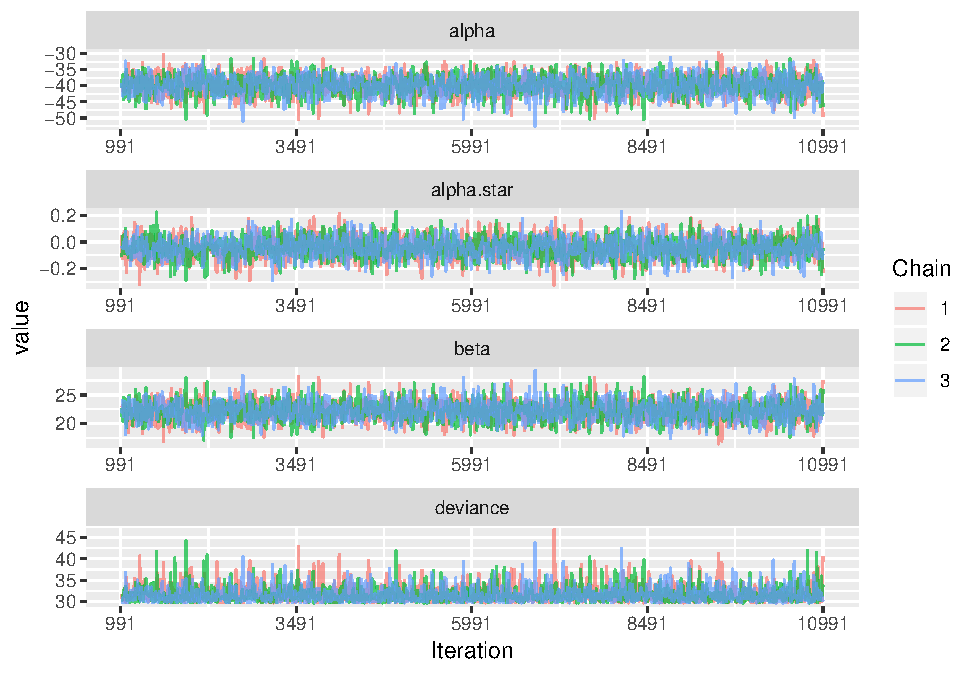
\includegraphics{FinalProject-SDSII_files/figure-latex/unnamed-chunk-25-1.pdf}

\begin{Shaded}
\begin{Highlighting}[]
\KeywordTok{ggs_running}\NormalTok{(chain_print)}
\end{Highlighting}
\end{Shaded}

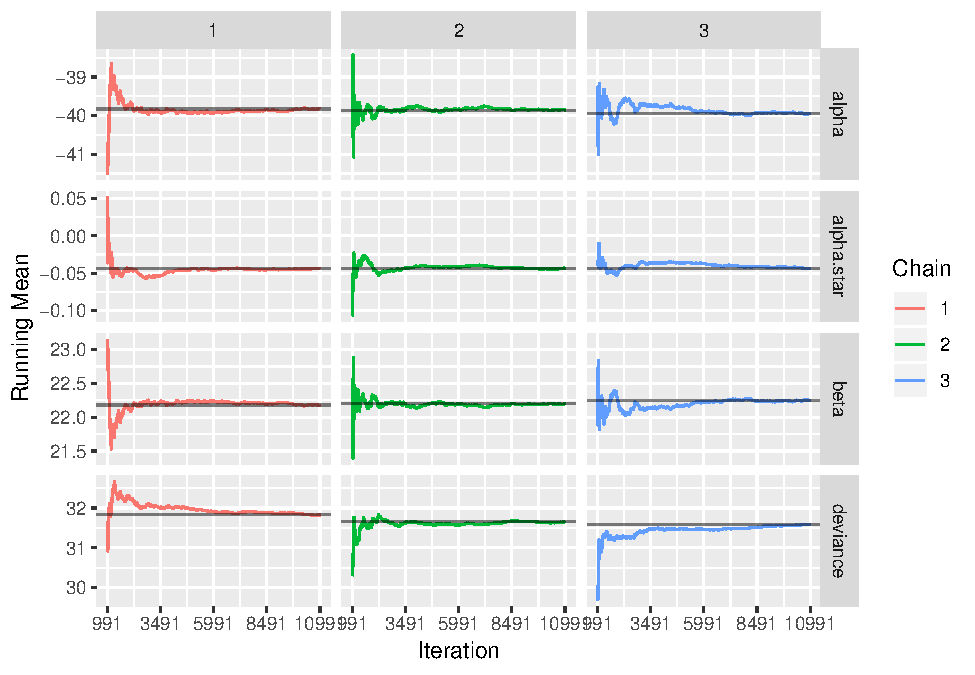
\includegraphics{FinalProject-SDSII_files/figure-latex/unnamed-chunk-25-2.pdf}

\begin{Shaded}
\begin{Highlighting}[]
\KeywordTok{ggs_autocorrelation}\NormalTok{(chain_print, }\DataTypeTok{nLags =} \DecValTok{30}\NormalTok{)}
\end{Highlighting}
\end{Shaded}

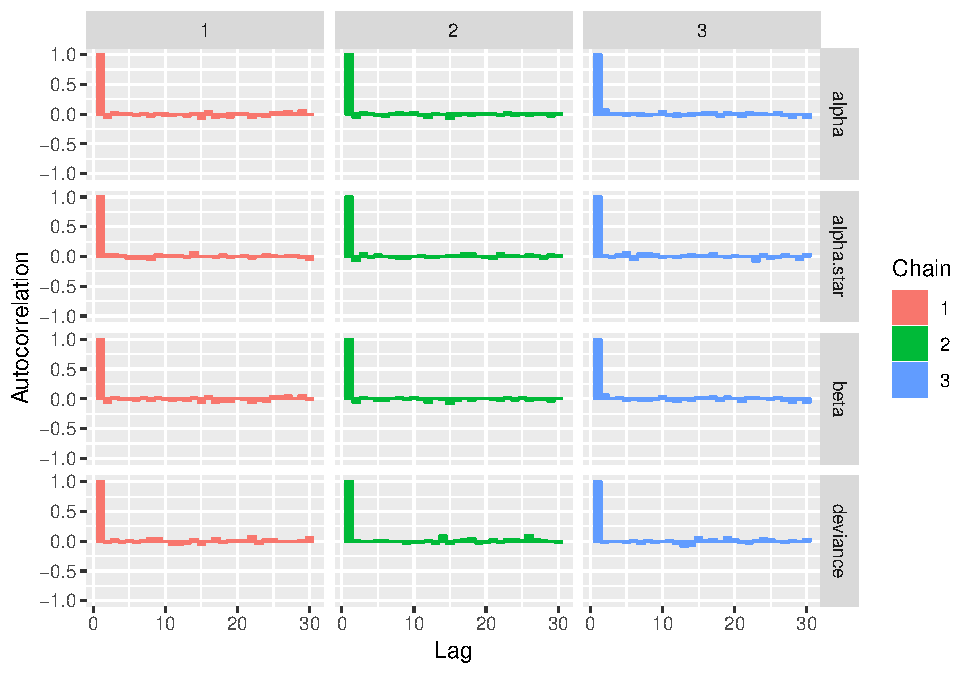
\includegraphics{FinalProject-SDSII_files/figure-latex/unnamed-chunk-25-3.pdf}
The plots of the chains don't seem to follow any pattern, the parameters
mean seems to converge and the autocorrelation has values very close to
zero after the first few iterations: all this indicates that the chains
converges properly. Finally, let's have a look at the estimated density
of the estimators:

\begin{Shaded}
\begin{Highlighting}[]
\KeywordTok{ggs_density}\NormalTok{(chain_print)}
\end{Highlighting}
\end{Shaded}

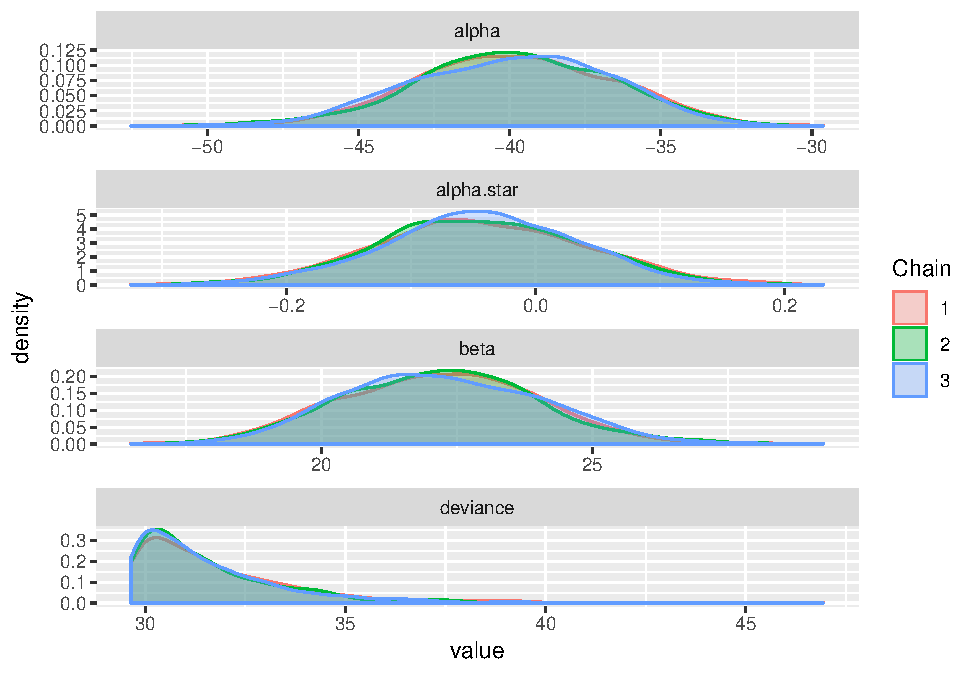
\includegraphics{FinalProject-SDSII_files/figure-latex/unnamed-chunk-26-1.pdf}
Smooth, unimodal and almost identical between the chains, we can be
confident in saying that all the chains converges.

Let's have now a look at the goodness of fit of our estimate:

\begin{Shaded}
\begin{Highlighting}[]
\KeywordTok{print}\NormalTok{(mcmc_res}\OperatorTok{$}\NormalTok{BUGSoutput}\OperatorTok{$}\NormalTok{summary[}\DecValTok{1}\OperatorTok{:}\DecValTok{4}\NormalTok{,}\KeywordTok{c}\NormalTok{(}\DecValTok{1}\OperatorTok{:}\DecValTok{3}\NormalTok{,}\DecValTok{7}\NormalTok{)])}
\end{Highlighting}
\end{Shaded}

\begin{verbatim}
##                    mean         sd        2.5%       97.5%
## alpha      -39.87974197 3.25428612 -46.3453158 -33.9393451
## alpha.star  -0.04365802 0.08170396  -0.2031907   0.1136823
## beta        22.21229433 1.80758010  18.9117051  25.8057077
## deviance    31.69079795 2.00252570  29.7050936  37.1199464
\end{verbatim}

\begin{Shaded}
\begin{Highlighting}[]
\NormalTok{alpha <-}\KeywordTok{as.numeric}\NormalTok{(mcmc_res}\OperatorTok{$}\NormalTok{BUGSoutput}\OperatorTok{$}\NormalTok{mean}\OperatorTok{$}\NormalTok{alpha) }
\NormalTok{beta <-}\StringTok{ }\KeywordTok{as.numeric}\NormalTok{(mcmc_res}\OperatorTok{$}\NormalTok{BUGSoutput}\OperatorTok{$}\NormalTok{mean}\OperatorTok{$}\NormalTok{beta)}

\KeywordTok{plot}\NormalTok{(}\DataTypeTok{x =}\NormalTok{ data}\OperatorTok{$}\NormalTok{x, }\DataTypeTok{y =}\NormalTok{ (data}\OperatorTok{$}\NormalTok{r}\OperatorTok{/}\NormalTok{data}\OperatorTok{$}\NormalTok{n), }
     \DataTypeTok{main =} \StringTok{"Beetles death rate - Extreme values model"}\NormalTok{,}
     \DataTypeTok{xlab =} \StringTok{"Concentration of carbon disulphide"}\NormalTok{, }
     \DataTypeTok{ylab =} \StringTok{"Beetles death rate"}\NormalTok{,}
     \DataTypeTok{pch =} \DecValTok{16}\NormalTok{, }\DataTypeTok{col =} \StringTok{"royalblue2"}\NormalTok{)}

\NormalTok{cloglog <-}\StringTok{ }\ControlFlowTok{function}\NormalTok{(x, a, b) }\KeywordTok{return}\NormalTok{(}\DecValTok{1}\OperatorTok{-}\KeywordTok{exp}\NormalTok{(}\OperatorTok{-}\KeywordTok{exp}\NormalTok{(a}\OperatorTok{+}\NormalTok{b }\OperatorTok{*}\StringTok{ }\NormalTok{x)))}

\KeywordTok{curve}\NormalTok{(}\KeywordTok{cloglog}\NormalTok{(x, alpha, beta), }\DataTypeTok{add =}\NormalTok{ T, }\DataTypeTok{col =} \StringTok{'red2'}\NormalTok{, }\DataTypeTok{lwd =} \FloatTok{1.5}\NormalTok{)}
\end{Highlighting}
\end{Shaded}

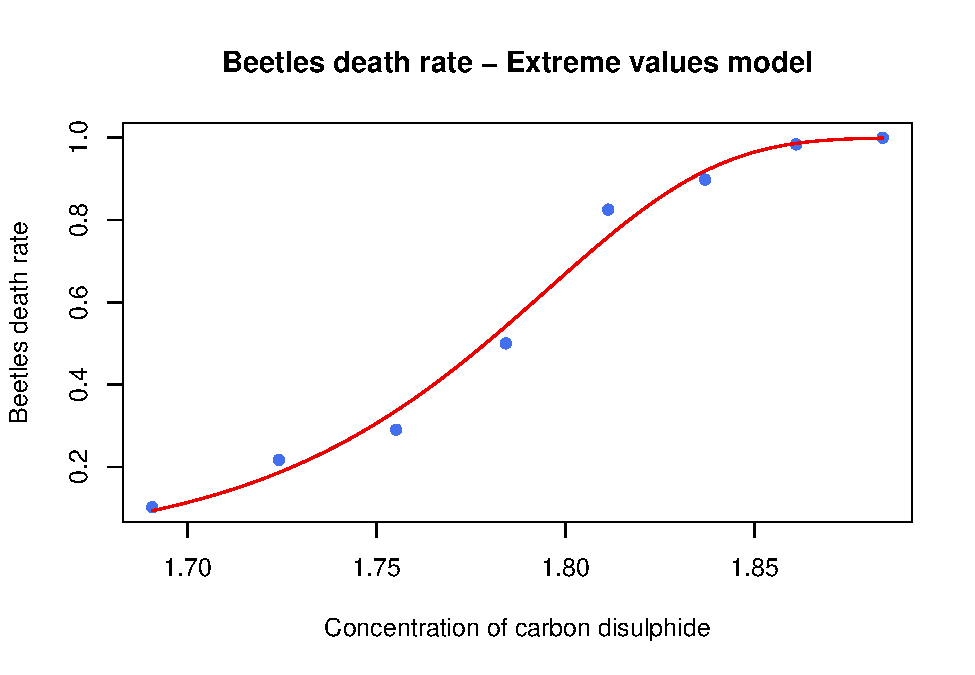
\includegraphics{FinalProject-SDSII_files/figure-latex/unnamed-chunk-28-1.pdf}

As we did before, we want to check also the confidence intervals:

\begin{Shaded}
\begin{Highlighting}[]
\NormalTok{alpha25 <-}\KeywordTok{as.numeric}\NormalTok{(mcmc_res}\OperatorTok{$}\NormalTok{BUGSoutput}\OperatorTok{$}\NormalTok{summary[}\DecValTok{1}\NormalTok{,}\DecValTok{3}\NormalTok{]) }
\NormalTok{beta25 <-}\StringTok{ }\KeywordTok{as.numeric}\NormalTok{(mcmc_res}\OperatorTok{$}\NormalTok{BUGSoutput}\OperatorTok{$}\NormalTok{summary[}\DecValTok{3}\NormalTok{,}\DecValTok{3}\NormalTok{])}
\NormalTok{alpha975 <-}\KeywordTok{as.numeric}\NormalTok{(mcmc_res}\OperatorTok{$}\NormalTok{BUGSoutput}\OperatorTok{$}\NormalTok{summary[}\DecValTok{1}\NormalTok{,}\DecValTok{7}\NormalTok{]) }
\NormalTok{beta975 <-}\StringTok{ }\KeywordTok{as.numeric}\NormalTok{(mcmc_res}\OperatorTok{$}\NormalTok{BUGSoutput}\OperatorTok{$}\NormalTok{summary[}\DecValTok{3}\NormalTok{,}\DecValTok{7}\NormalTok{])}

\KeywordTok{plot}\NormalTok{(}\DataTypeTok{x =}\NormalTok{ data}\OperatorTok{$}\NormalTok{x, }\DataTypeTok{y =}\NormalTok{ (data}\OperatorTok{$}\NormalTok{r}\OperatorTok{/}\NormalTok{data}\OperatorTok{$}\NormalTok{n), }
     \DataTypeTok{main =} \StringTok{"Beetles death rate - Extreme values model confidence intervals"}\NormalTok{,}
     \DataTypeTok{xlab =} \StringTok{"Concentration of carbon disulphide"}\NormalTok{, }
     \DataTypeTok{ylab =} \StringTok{"Beetles death rate"}\NormalTok{,}
     \DataTypeTok{pch =} \DecValTok{16}\NormalTok{, }\DataTypeTok{col =} \StringTok{"royalblue2"}\NormalTok{, }\DataTypeTok{xlim =} \KeywordTok{c}\NormalTok{(}\DecValTok{1}\NormalTok{,}\FloatTok{2.6}\NormalTok{))}

\KeywordTok{curve}\NormalTok{(}\KeywordTok{cloglog}\NormalTok{(x, alpha, beta), }\DataTypeTok{add =}\NormalTok{ T, }\DataTypeTok{col =} \StringTok{'red2'}\NormalTok{, }\DataTypeTok{lwd =} \FloatTok{1.5}\NormalTok{)}
\KeywordTok{curve}\NormalTok{(}\KeywordTok{cloglog}\NormalTok{(x, alpha25, beta25), }\DataTypeTok{add =}\NormalTok{ T, }\DataTypeTok{lwd =} \DecValTok{1}\NormalTok{, }\DataTypeTok{lty =} \DecValTok{2}\NormalTok{, }\DataTypeTok{col =} \StringTok{'azure4'}\NormalTok{)}
\KeywordTok{curve}\NormalTok{(}\KeywordTok{cloglog}\NormalTok{(x, alpha975, beta975), }\DataTypeTok{add =}\NormalTok{ T, }\DataTypeTok{lwd =} \DecValTok{1}\NormalTok{, }\DataTypeTok{lty =} \DecValTok{2}\NormalTok{, }\DataTypeTok{col =} \StringTok{'azure4'}\NormalTok{)}
\end{Highlighting}
\end{Shaded}

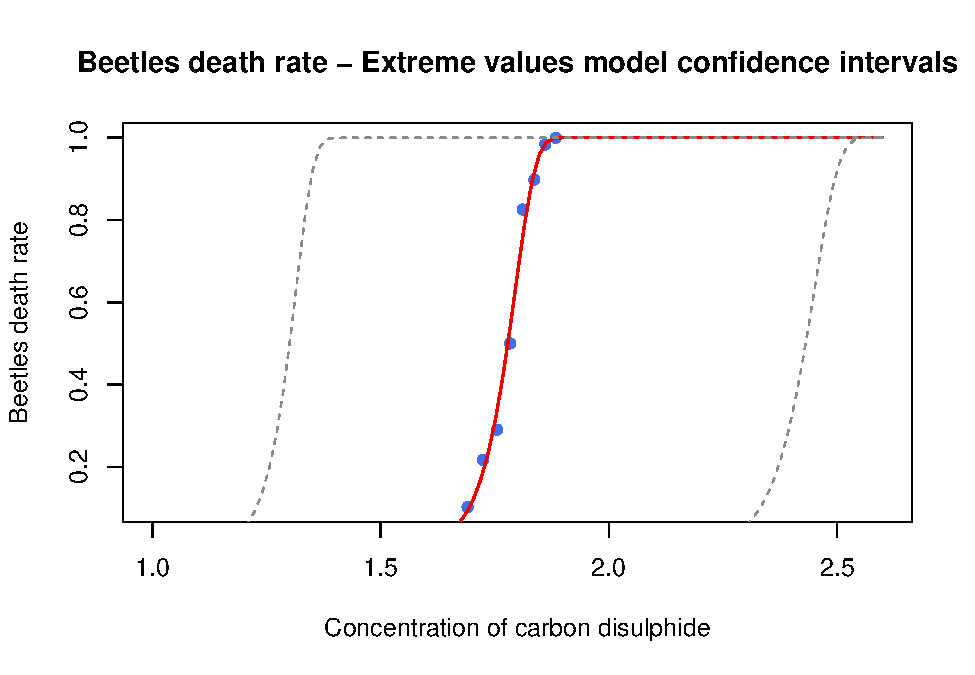
\includegraphics{FinalProject-SDSII_files/figure-latex/unnamed-chunk-29-1.pdf}

\hypertarget{comparison-with-frequentist-inference}{%
\section{Comparison with frequentist
inference}\label{comparison-with-frequentist-inference}}

When we want to compare the different results between frequentist
approach and Bayesian approach, we have to keep in mind first the
differences between the two philosophies of the approaches. In the
frequentist approach we use the likelihood function to get
\(P(D| \theta, M)\), meanwhile in the Bayesian approach we are looking
for the probability of the model parameters \(P(\theta| D, M)\). So we
can say that the frequentists operate on the probability of the data,
while the Bayesian operate on a probability of the model parameters. So
what is done in the frequentist approach, is to compute the likelihood
directly from the model, and by optimizinge this likelihood expression
directly, it's possible to arrive a t an estimated best model fit.
Bayesian, on the other hand, have a slightly more difficult task that
involves the priors beliefs. In situations where the model doesn't
belong to twell known parametric families, it's much difficult to
evaluate the simple formula of the postirior, so we have to use more
advanced techniques, such as Markov Chain Monte Carlo.

To arrange the comparison, the first step to do is to find the optimal
parameters of the likelihood (Maximum Likelihood Estimation), as
required in the frequentist approach. We will use the GLM (General
Linear Methods) library built-in in R:

\begin{Shaded}
\begin{Highlighting}[]
\NormalTok{logit_freq <-}\StringTok{ }\KeywordTok{glm}\NormalTok{(Rate }\OperatorTok{~}\StringTok{ }\NormalTok{Concentration, }\DataTypeTok{family =} \KeywordTok{binomial}\NormalTok{(}\DataTypeTok{link =} \StringTok{"logit"}\NormalTok{), }\DataTypeTok{data =}\NormalTok{ df)}
\NormalTok{probit_freq <-}\StringTok{ }\KeywordTok{glm}\NormalTok{(Rate }\OperatorTok{~}\StringTok{ }\NormalTok{Concentration, }\DataTypeTok{family =} \KeywordTok{binomial}\NormalTok{(}\DataTypeTok{link =} \StringTok{"probit"}\NormalTok{), }\DataTypeTok{data =}\NormalTok{ df)}
\NormalTok{cloglog_freq <-}\StringTok{ }\KeywordTok{glm}\NormalTok{(Rate }\OperatorTok{~}\StringTok{ }\NormalTok{Concentration, }\DataTypeTok{family =} \KeywordTok{binomial}\NormalTok{(}\DataTypeTok{link =} \StringTok{"cloglog"}\NormalTok{), }\DataTypeTok{data =}\NormalTok{ df)}
\end{Highlighting}
\end{Shaded}

After we prepared the models, it's time to have a look at the results.
First we want to observe how much the frequentist results differs from
the bayesian ones:

\begin{Shaded}
\begin{Highlighting}[]
\NormalTok{toprint =}\StringTok{ }\KeywordTok{as.data.frame}\NormalTok{(}\KeywordTok{list}\NormalTok{(}\StringTok{"Concentration"}\NormalTok{ =}\StringTok{ }\NormalTok{data}\OperatorTok{$}\NormalTok{x, }
                        \StringTok{"Number_of_beetles"}\NormalTok{ =}\StringTok{ }\NormalTok{data}\OperatorTok{$}\NormalTok{n, }
                        \StringTok{"Number_killed"}\NormalTok{ =}\StringTok{ }\NormalTok{data}\OperatorTok{$}\NormalTok{r))}

\NormalTok{comp_res <-}\StringTok{ }\KeywordTok{as.data.frame}\NormalTok{(}\KeywordTok{matrix}\NormalTok{(}\KeywordTok{as.numeric}\NormalTok{(}\KeywordTok{list}\NormalTok{(}
\NormalTok{                               logit_res}\OperatorTok{$}\NormalTok{BUGSoutput}\OperatorTok{$}\NormalTok{mean}\OperatorTok{$}\NormalTok{alpha,}
\NormalTok{                               logit_res}\OperatorTok{$}\NormalTok{BUGSoutput}\OperatorTok{$}\NormalTok{mean}\OperatorTok{$}\NormalTok{beta,}
\NormalTok{                               logit_freq}\OperatorTok{$}\NormalTok{coefficients[}\DecValTok{1}\NormalTok{],}
\NormalTok{                               logit_freq}\OperatorTok{$}\NormalTok{coefficients[}\DecValTok{2}\NormalTok{],}
\NormalTok{                               probit_res}\OperatorTok{$}\NormalTok{BUGSoutput}\OperatorTok{$}\NormalTok{mean}\OperatorTok{$}\NormalTok{alpha,}
\NormalTok{                               probit_res}\OperatorTok{$}\NormalTok{BUGSoutput}\OperatorTok{$}\NormalTok{mean}\OperatorTok{$}\NormalTok{beta,}
\NormalTok{                               probit_freq}\OperatorTok{$}\NormalTok{coefficients[}\DecValTok{1}\NormalTok{],}
\NormalTok{                               probit_freq}\OperatorTok{$}\NormalTok{coefficients[}\DecValTok{2}\NormalTok{],}
\NormalTok{                               cloglog_res}\OperatorTok{$}\NormalTok{BUGSoutput}\OperatorTok{$}\NormalTok{mean}\OperatorTok{$}\NormalTok{alpha,}
\NormalTok{                               cloglog_res}\OperatorTok{$}\NormalTok{BUGSoutput}\OperatorTok{$}\NormalTok{mean}\OperatorTok{$}\NormalTok{beta,}
\NormalTok{                               cloglog_freq}\OperatorTok{$}\NormalTok{coefficients[}\DecValTok{1}\NormalTok{],}
\NormalTok{                               cloglog_freq}\OperatorTok{$}\NormalTok{coefficients[}\DecValTok{2}\NormalTok{])), }\DataTypeTok{nrow =} \DecValTok{2}\NormalTok{, }\DataTypeTok{ncol =} \DecValTok{6}\NormalTok{))}
\KeywordTok{names}\NormalTok{(comp_res) <-}\StringTok{ }\KeywordTok{rep}\NormalTok{(}\KeywordTok{c}\NormalTok{(}\StringTok{'Post.'}\NormalTok{, }\StringTok{'MLE'}\NormalTok{), }\DecValTok{3}\NormalTok{)}
\KeywordTok{row.names}\NormalTok{(comp_res) <-}\StringTok{ }\KeywordTok{c}\NormalTok{(}\StringTok{'alpha'}\NormalTok{, }\StringTok{'beta'}\NormalTok{)}

\KeywordTok{kable}\NormalTok{(comp_res, }\StringTok{"latex"}\NormalTok{, }\DataTypeTok{booktabs =}\NormalTok{ T) }\OperatorTok
\StringTok{  }\KeywordTok{kable_styling}\NormalTok{(}\DataTypeTok{latex_options =}\KeywordTok{c}\NormalTok{(}\StringTok{"striped"}\NormalTok{, }\StringTok{"hold_position"}\NormalTok{)) }\OperatorTok
\StringTok{  }\KeywordTok{add_header_above}\NormalTok{(}\KeywordTok{c}\NormalTok{(}\StringTok{" "}\NormalTok{, }\StringTok{"Logistic"}\NormalTok{ =}\StringTok{ }\DecValTok{2}\NormalTok{, }\StringTok{"Probit"}\NormalTok{ =}\StringTok{ }\DecValTok{2}\NormalTok{, }\StringTok{"Extreme values"}\NormalTok{ =}\StringTok{ }\DecValTok{2}\NormalTok{))}
\end{Highlighting}
\end{Shaded}

\begin{table}[!h]
\centering
\begin{tabular}{lrrrrrr}
\toprule
\multicolumn{1}{c}{ } & \multicolumn{2}{c}{Logistic} & \multicolumn{2}{c}{Probit} & \multicolumn{2}{c}{Extreme values} \\
\cmidrule(l{3pt}r{3pt}){2-3} \cmidrule(l{3pt}r{3pt}){4-5} \cmidrule(l{3pt}r{3pt}){6-7}
  & Post. & MLE & Post. & MLE & Post. & MLE\\
\midrule
\rowcolor{gray!6}  alpha & -61.19868 & -60.45910 & -35.17028 & -34.80375 & -39.87974 & -39.53294\\
beta & 34.54274 & 34.12134 & 19.86110 & 19.65214 & 22.21229 & 22.01742\\
\bottomrule
\end{tabular}
\end{table}

What we can see is that, for all the three models, the results between
bayesian and frequentist approaches do not differ from each other. In
fact it's not possible to see any major difference between the results,
which does not give us space to have a toughtful considerations on the
differences in between these two approaches, in this specific case. What
we can do for the frequentist approach (and we will do the same also for
the bayesian in the next section) is to compare the goodness of fit of
the three models. To do so, we will use the Akaike information criterion
(AIC), already computed by default from the \emph{glm} function in R.

The AIC is an estimator of the relative quality of statistical models
for a given set of data. The formula to compute it is the following:
\[ AIC = 2k -2ln(\hat{L})\] where \emph{k} is the number of estimated
parameters of the model, and \(\hat{L}\) is the maximum value of the
log-likelihood. Hence, a good model must have a good trade-off between
these two values. Obviously, the lowest the AIC, the better the model.
It is important to remember that, unlike adjusted R-squared, the number
itself is not meaningful. So it is useful for comparing models, but it
is not interpretable on its own. What we are looking for is the model
with the lowest AIC, which is indicating the best fitting model:

\begin{Shaded}
\begin{Highlighting}[]
\NormalTok{toprint <-}\StringTok{ }\KeywordTok{as.data.frame}\NormalTok{(}\KeywordTok{matrix}\NormalTok{(}
                          \KeywordTok{as.numeric}\NormalTok{(}
                            \KeywordTok{list}\NormalTok{(}
\NormalTok{                              logit_freq}\OperatorTok{$}\NormalTok{aic, }
\NormalTok{                              probit_freq}\OperatorTok{$}\NormalTok{aic, }
\NormalTok{                              cloglog_freq}\OperatorTok{$}\NormalTok{aic)),}
                          \DataTypeTok{nrow =} \DecValTok{3}\NormalTok{, }\DataTypeTok{ncol =}\DecValTok{1}\NormalTok{))}
\KeywordTok{names}\NormalTok{(toprint) <-}\StringTok{ "AIC models comparison"}
\KeywordTok{row.names}\NormalTok{(toprint) <-}\StringTok{ }\KeywordTok{c}\NormalTok{(}\StringTok{'Logistic model: '}\NormalTok{, }\StringTok{'Probit model: '}\NormalTok{, }\StringTok{"Extreme values model: "}\NormalTok{)}
\KeywordTok{kable}\NormalTok{(toprint, }\StringTok{"latex"}\NormalTok{, }\DataTypeTok{booktabs =}\NormalTok{ T) }\OperatorTok
\StringTok{  }\KeywordTok{kable_styling}\NormalTok{(}\DataTypeTok{latex_options =}\KeywordTok{c}\NormalTok{(}\StringTok{"striped"}\NormalTok{, }\StringTok{"hold_position"}\NormalTok{))}
\end{Highlighting}
\end{Shaded}

\begin{table}[!h]
\centering
\begin{tabular}{lr}
\toprule
  & AIC models comparison\\
\midrule
\rowcolor{gray!6}  Logistic model: & 8.033914\\
Probit model: & 8.099567\\
\rowcolor{gray!6}  Extreme values model: & 7.757714\\
\bottomrule
\end{tabular}
\end{table}

As is possible to observe, al the three AIC values seems to be fairly
close to each other, having the Extreme Values model with the lowest
value, which indicates that for this data, it seems the best fitting
model.

\hypertarget{bayesian-model-comparison}{%
\section{Bayesian model comparison}\label{bayesian-model-comparison}}

Once we did the comparison between frequentist and bayesian worlds (and
inside the frequentist itself), it is time to compare the models with
the parameters we obtained through bayesian inference. We can start by
plotting all the models together, to have a visual comprehension of
them:

\begin{Shaded}
\begin{Highlighting}[]
\NormalTok{comp_res <-}\StringTok{ }\KeywordTok{as.data.frame}\NormalTok{(}\KeywordTok{matrix}\NormalTok{(}\KeywordTok{as.numeric}\NormalTok{(}\KeywordTok{list}\NormalTok{(}
\NormalTok{                               logit_res}\OperatorTok{$}\NormalTok{BUGSoutput}\OperatorTok{$}\NormalTok{mean}\OperatorTok{$}\NormalTok{alpha,}
\NormalTok{                               logit_res}\OperatorTok{$}\NormalTok{BUGSoutput}\OperatorTok{$}\NormalTok{mean}\OperatorTok{$}\NormalTok{beta,}
\NormalTok{                               probit_res}\OperatorTok{$}\NormalTok{BUGSoutput}\OperatorTok{$}\NormalTok{mean}\OperatorTok{$}\NormalTok{alpha,}
\NormalTok{                               probit_res}\OperatorTok{$}\NormalTok{BUGSoutput}\OperatorTok{$}\NormalTok{mean}\OperatorTok{$}\NormalTok{beta,}
\NormalTok{                               cloglog_res}\OperatorTok{$}\NormalTok{BUGSoutput}\OperatorTok{$}\NormalTok{mean}\OperatorTok{$}\NormalTok{alpha,}
\NormalTok{                               cloglog_res}\OperatorTok{$}\NormalTok{BUGSoutput}\OperatorTok{$}\NormalTok{mean}\OperatorTok{$}\NormalTok{beta)), }\DataTypeTok{nrow =} \DecValTok{2}\NormalTok{, }\DataTypeTok{ncol =} \DecValTok{3}\NormalTok{))}
\KeywordTok{names}\NormalTok{(comp_res) <-}\StringTok{ }\KeywordTok{c}\NormalTok{(}\StringTok{'logit'}\NormalTok{, }\StringTok{'probit'}\NormalTok{, }\StringTok{"cloglog"}\NormalTok{)}
\KeywordTok{row.names}\NormalTok{(comp_res) <-}\StringTok{ }\KeywordTok{c}\NormalTok{(}\StringTok{'alpha'}\NormalTok{, }\StringTok{'beta'}\NormalTok{)}


\KeywordTok{plot}\NormalTok{(}\DataTypeTok{x =}\NormalTok{ data}\OperatorTok{$}\NormalTok{x, }\DataTypeTok{y =}\NormalTok{ (data}\OperatorTok{$}\NormalTok{r}\OperatorTok{/}\NormalTok{data}\OperatorTok{$}\NormalTok{n), }
     \DataTypeTok{main =} \StringTok{"Beetles death rate - Extreme values model confidence intervals"}\NormalTok{,}
     \DataTypeTok{xlab =} \StringTok{"Concentration of carbon disulphide"}\NormalTok{, }
     \DataTypeTok{ylab =} \StringTok{"Beetles death rate"}\NormalTok{, }\DataTypeTok{col =} \StringTok{'black'}\NormalTok{,}
     \DataTypeTok{pch =} \DecValTok{16}\NormalTok{)}

\KeywordTok{curve}\NormalTok{(}\KeywordTok{logit}\NormalTok{(x, comp_res[}\StringTok{'alpha'}\NormalTok{,}\StringTok{'logit'}\NormalTok{], comp_res[}\StringTok{'beta'}\NormalTok{,}\StringTok{'logit'}\NormalTok{]), }\DataTypeTok{add =}\NormalTok{ T, }
      \DataTypeTok{col =} \StringTok{'firebrick3'}\NormalTok{, }\DataTypeTok{lwd =} \FloatTok{1.5}\NormalTok{)}
\KeywordTok{curve}\NormalTok{(}\KeywordTok{pnorm}\NormalTok{(comp_res[}\StringTok{'alpha'}\NormalTok{,}\StringTok{'probit'}\NormalTok{] }\OperatorTok{+}\StringTok{ }\NormalTok{(comp_res[}\StringTok{'beta'}\NormalTok{,}\StringTok{'probit'}\NormalTok{] }\OperatorTok{*}\StringTok{ }\NormalTok{x), }\DataTypeTok{mean =} \DecValTok{0}\NormalTok{, }
            \DataTypeTok{sd =} \DecValTok{1}\NormalTok{, }\DataTypeTok{lower.tail =} \OtherTok{TRUE}\NormalTok{), }\DataTypeTok{add =}\NormalTok{ T, }\DataTypeTok{col =} \StringTok{'seagreen4'}\NormalTok{, }\DataTypeTok{lwd =} \FloatTok{1.5}\NormalTok{)}
\KeywordTok{curve}\NormalTok{(}\KeywordTok{cloglog}\NormalTok{(x, comp_res[}\StringTok{'alpha'}\NormalTok{,}\StringTok{'cloglog'}\NormalTok{], comp_res[}\StringTok{'beta'}\NormalTok{,}\StringTok{'cloglog'}\NormalTok{]), }\DataTypeTok{add =}\NormalTok{ T, }
      \DataTypeTok{col =} \StringTok{'dodgerblue4'}\NormalTok{, }\DataTypeTok{lwd =} \FloatTok{1.5}\NormalTok{)}
\KeywordTok{legend}\NormalTok{(}\DecValTok{1}\NormalTok{, }\DecValTok{95}\NormalTok{, }\DataTypeTok{legend=}\KeywordTok{c}\NormalTok{(}\StringTok{"Logistic"}\NormalTok{, }\StringTok{"Probit"}\NormalTok{, }\StringTok{"Extreme values"}\NormalTok{), }
       \DataTypeTok{col=}\KeywordTok{c}\NormalTok{(}\StringTok{"firebrick3"}\NormalTok{, }\StringTok{"seagreen4"}\NormalTok{, }\StringTok{"dodgerblue4"}\NormalTok{), }\DataTypeTok{lty=}\DecValTok{1}\OperatorTok{:}\DecValTok{2}\NormalTok{, }\DataTypeTok{cex=}\FloatTok{0.8}\NormalTok{)}
\KeywordTok{legend}\NormalTok{(}\StringTok{"topleft"}\NormalTok{, }\DataTypeTok{legend=}\KeywordTok{c}\NormalTok{(}\StringTok{"Logistic"}\NormalTok{, }\StringTok{"Probit"}\NormalTok{, }\StringTok{"Extreme values"}\NormalTok{), }
       \DataTypeTok{col=}\KeywordTok{c}\NormalTok{(}\StringTok{"firebrick3"}\NormalTok{, }\StringTok{"seagreen4"}\NormalTok{, }\StringTok{"dodgerblue4"}\NormalTok{),  }\DataTypeTok{lty=}\DecValTok{1}\NormalTok{, }\DataTypeTok{lwd =} \DecValTok{4}\NormalTok{)}
\end{Highlighting}
\end{Shaded}

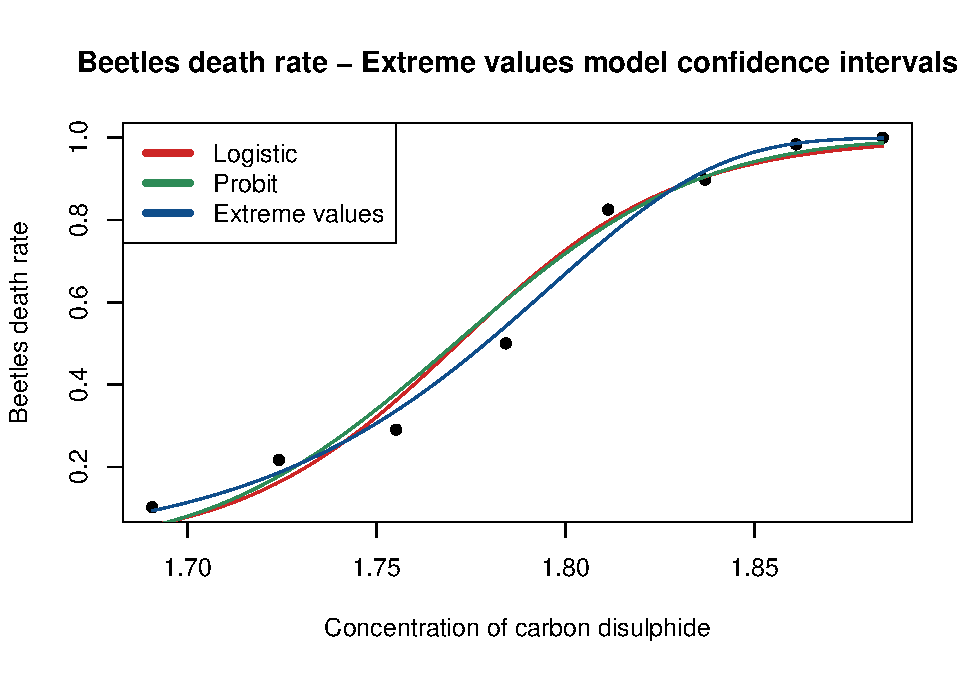
\includegraphics{FinalProject-SDSII_files/figure-latex/unnamed-chunk-33-1.pdf}
As we can observe, from the plot itself it is very difficult to identify
which model fits the best our data. In this case, as we did before in
the frequentist case, we will need to use an Information Criteria to
evaluate how well the model fit the data, in this case the DIC.\\
The deviance information criterion (DIC) was introduced by
\emph{Spiegelhalter et al.~(2002)} as a measure of model comparison and
adequacy. It is given by the expression
\[DIC(m) = 2\overline{D(\theta_m,m)} - D(\overline{\theta}_m,m) = D(\overline{\theta}_m,m) + 2p_m\]
where \(D(\overline{\theta}_m,m)\) is the usual deviance measure, which
is equal to minus twice the log-likelihood:
\[D(\theta_m,m) = -2log \:f(y|\theta_m, m)\] and
\(\overline{D(\theta_m,m)}\) is its posterior mean, \(p_m\), can be
interpeted as the number of ``effective'' parameters form model \(m\)
given by \[p_m = \overline{D(\theta_m,m)} -  D(\overline{\theta}_m,m)\]
and \(\overline{\theta}_m\) is the posterior mean of the parameters
involved in the model \(m\).\\
So we will have that smalle DIC values indicate a better-fittinf model.
DIC must be used with caution since it assumes that the posterior mean
can be used as a ``good'' summary of central location for description of
the posterior distribution.\\
Generally DIC is considered as a generalization of AIC. In simple
one-stage models, AIC and DIC are identical. But, like in our case,
differences occur in hierarchical and latent variable models where DIC
uses the number of ``effective'' parameters instead of the actual number
of parameters used by AIC. This is the reason why, in this kind of
analysis was not possible for us to compare the AIC results of the
frequentist analysis with the DIC results we will compare now, from the
bayesian analysis. So again, as we saw previously with the AIC, the idea
is that the model with a smaller DIC is preferable to a model having a
larger DIC. Also here, the concept is to have a good trade-off between
number of parametrs to estimate, and the deviance of the model (instead
the likelihood, as in the AIC).\\
Let's have a look at the DIC values we obtained from the run of the
chains:

\begin{Shaded}
\begin{Highlighting}[]
\NormalTok{toprint <-}\StringTok{ }\KeywordTok{as.data.frame}\NormalTok{(}\KeywordTok{matrix}\NormalTok{(}
                          \KeywordTok{as.numeric}\NormalTok{(}
                            \KeywordTok{list}\NormalTok{(}
\NormalTok{                              logit_res}\OperatorTok{$}\NormalTok{BUGSoutput}\OperatorTok{$}\NormalTok{DIC, }
\NormalTok{                              probit_res}\OperatorTok{$}\NormalTok{BUGSoutput}\OperatorTok{$}\NormalTok{DIC, }
\NormalTok{                              cloglog_res}\OperatorTok{$}\NormalTok{BUGSoutput}\OperatorTok{$}\NormalTok{DIC)),}
                          \DataTypeTok{nrow =} \DecValTok{3}\NormalTok{, }\DataTypeTok{ncol =}\DecValTok{1}\NormalTok{))}
\KeywordTok{names}\NormalTok{(toprint) <-}\StringTok{ "DIC models comparison"}
\KeywordTok{row.names}\NormalTok{(toprint) <-}\StringTok{ }\KeywordTok{c}\NormalTok{(}\StringTok{'Logistic model: '}\NormalTok{, }\StringTok{'Probit model: '}\NormalTok{, }\StringTok{"Extreme values model: "}\NormalTok{)}
\KeywordTok{kable}\NormalTok{(toprint, }\StringTok{"latex"}\NormalTok{, }\DataTypeTok{booktabs =}\NormalTok{ T) }\OperatorTok
\StringTok{  }\KeywordTok{kable_styling}\NormalTok{(}\DataTypeTok{latex_options =}\KeywordTok{c}\NormalTok{(}\StringTok{"striped"}\NormalTok{, }\StringTok{"hold_position"}\NormalTok{))}
\end{Highlighting}
\end{Shaded}

\begin{table}[!h]
\centering
\begin{tabular}{lr}
\toprule
  & DIC models comparison\\
\midrule
\rowcolor{gray!6}  Logistic model: & 126.86158\\
Probit model: & 40.42298\\
\rowcolor{gray!6}  Extreme values model: & 33.69169\\
\bottomrule
\end{tabular}
\end{table}

As is possible to see, the model that seems to have the best goodness of
fit is again the extreme values model. This match the results of the
frequentist analysis, confirming that the extreme values model is the
one that is most suitable for our data, probably due to a smaller
discrepancy between observed and predicted values.

Since we want to go a little bit deeper with the comparison, it is
useful to have a comparison done by generating new data from a new
distribution proposed by us. The models will then be tested again, in
light of the new data, to see if they can recover the structure of the
resampled data. We do this with the aim to understand if the
performances of the proposed models are due to randomness or the model
can generalize well any combination of parameters.

The first step taken was the generation of new dataset, from existing
models: we generated 300 different datasets, and for each, all the three
model proposed where fitted. The first 100 datasets are generated from a
logistic model, another batch of 100 datasets using the probit model and
the last 100 datasets using the extreme values model.

Let's start with the logit model:

\begin{Shaded}
\begin{Highlighting}[]
\NormalTok{n_data =}\StringTok{ }\DecValTok{100}
\NormalTok{res <-}\StringTok{ }\KeywordTok{matrix}\NormalTok{(}\KeywordTok{rep}\NormalTok{(}\OtherTok{NA}\NormalTok{,n_data}\OperatorTok{*}\DecValTok{3}\OperatorTok{*}\DecValTok{3}\NormalTok{), }\DataTypeTok{nrow =}\NormalTok{ n_data, }\DataTypeTok{ncol =} \DecValTok{9}\NormalTok{)}
\KeywordTok{colnames}\NormalTok{(res) <-}\StringTok{ }\KeywordTok{c}\NormalTok{(}\StringTok{'logit_alpha'}\NormalTok{,}\StringTok{'logit_beta'}\NormalTok{,}\StringTok{'logit_DIC'}\NormalTok{,}
                   \StringTok{'probit_alpha'}\NormalTok{,}\StringTok{'probit_beta'}\NormalTok{,}\StringTok{'probit_DIC'}\NormalTok{,}
                   \StringTok{'cloglog_alpha'}\NormalTok{,}\StringTok{'cloglog_beta'}\NormalTok{,}\StringTok{'cloglog_DIC'}\NormalTok{)}
\NormalTok{a <-}\StringTok{ }\NormalTok{logit_res}\OperatorTok{$}\NormalTok{BUGSoutput}\OperatorTok{$}\NormalTok{mean}\OperatorTok{$}\NormalTok{alpha}
\NormalTok{b <-}\StringTok{ }\NormalTok{logit_res}\OperatorTok{$}\NormalTok{BUGSoutput}\OperatorTok{$}\NormalTok{mean}\OperatorTok{$}\NormalTok{beta}

\ControlFlowTok{for}\NormalTok{(i }\ControlFlowTok{in} \DecValTok{1}\OperatorTok{:}\NormalTok{n_data)\{}
\NormalTok{  y_new =}\StringTok{ }\KeywordTok{rbinom}\NormalTok{(}\KeywordTok{length}\NormalTok{(data}\OperatorTok{$}\NormalTok{n), data}\OperatorTok{$}\NormalTok{n, }\KeywordTok{logit}\NormalTok{(data}\OperatorTok{$}\NormalTok{x, a, b))}

\NormalTok{  data.list=}\StringTok{ }\KeywordTok{list}\NormalTok{(}\DataTypeTok{r =}\NormalTok{ y_new,}
                \DataTypeTok{n =}\NormalTok{ data}\OperatorTok{$}\NormalTok{n,}
                \DataTypeTok{x =}\NormalTok{ data}\OperatorTok{$}\NormalTok{x,}
                \DataTypeTok{tau_alpha =}\NormalTok{ tau_alpha,}
                \DataTypeTok{tau_beta =}\NormalTok{ tau_beta,}
                \DataTypeTok{N =} \DecValTok{8}\NormalTok{)}
  
\NormalTok{  mcmc_res =}\StringTok{ }\KeywordTok{jags}\NormalTok{( }\DataTypeTok{model.file =} \KeywordTok{textConnection}\NormalTok{(model_}\DecValTok{1}\NormalTok{),}
                  \DataTypeTok{data =}\NormalTok{ data.list, }
                  \DataTypeTok{n.chains =} \DecValTok{3}\NormalTok{, }
                  \DataTypeTok{n.iter =} \DecValTok{11000}\NormalTok{, }
                  \DataTypeTok{n.burnin =} \DecValTok{1000}\NormalTok{,}
                  \DataTypeTok{inits =}\NormalTok{ init.list.nod, }
                  \DataTypeTok{parameters.to.save =} \KeywordTok{c}\NormalTok{(}\StringTok{"alpha"}\NormalTok{,}\StringTok{"alpha.star"}\NormalTok{,}\StringTok{"beta"}\NormalTok{))}
  
\NormalTok{  res[i, }\StringTok{'logit_alpha'}\NormalTok{] =}\StringTok{ }\NormalTok{mcmc_res}\OperatorTok{$}\NormalTok{BUGSoutput}\OperatorTok{$}\NormalTok{mean}\OperatorTok{$}\NormalTok{alpha}
\NormalTok{  res[i, }\StringTok{'logit_beta'}\NormalTok{] =}\StringTok{ }\NormalTok{mcmc_res}\OperatorTok{$}\NormalTok{BUGSoutput}\OperatorTok{$}\NormalTok{mean}\OperatorTok{$}\NormalTok{beta}
\NormalTok{  res[i, }\StringTok{'logit_DIC'}\NormalTok{] =}\StringTok{ }\NormalTok{mcmc_res}\OperatorTok{$}\NormalTok{BUGSoutput}\OperatorTok{$}\NormalTok{DIC}
  
\NormalTok{  mcmc_res =}\StringTok{ }\KeywordTok{jags}\NormalTok{( }\DataTypeTok{model.file =} \KeywordTok{textConnection}\NormalTok{(model_}\DecValTok{2}\NormalTok{),}
                  \DataTypeTok{data =}\NormalTok{ data.list, }
                  \DataTypeTok{n.chains =} \DecValTok{3}\NormalTok{, }
                  \DataTypeTok{n.iter =} \DecValTok{11000}\NormalTok{, }
                  \DataTypeTok{n.burnin =} \DecValTok{1000}\NormalTok{,}
                  \DataTypeTok{inits =}\NormalTok{ init.list.nod, }
                  \DataTypeTok{parameters.to.save =} \KeywordTok{c}\NormalTok{(}\StringTok{"alpha"}\NormalTok{,}\StringTok{"alpha.star"}\NormalTok{,}\StringTok{"beta"}\NormalTok{))}
  
\NormalTok{  res[i, }\StringTok{'probit_alpha'}\NormalTok{] =}\StringTok{ }\NormalTok{mcmc_res}\OperatorTok{$}\NormalTok{BUGSoutput}\OperatorTok{$}\NormalTok{mean}\OperatorTok{$}\NormalTok{alpha}
\NormalTok{  res[i, }\StringTok{'probit_beta'}\NormalTok{] =}\StringTok{ }\NormalTok{mcmc_res}\OperatorTok{$}\NormalTok{BUGSoutput}\OperatorTok{$}\NormalTok{mean}\OperatorTok{$}\NormalTok{beta}
\NormalTok{  res[i, }\StringTok{'probit_DIC'}\NormalTok{] =}\StringTok{ }\NormalTok{mcmc_res}\OperatorTok{$}\NormalTok{BUGSoutput}\OperatorTok{$}\NormalTok{DIC}
  
\NormalTok{  mcmc_res =}\StringTok{ }\KeywordTok{jags}\NormalTok{( }\DataTypeTok{model.file =} \KeywordTok{textConnection}\NormalTok{(model_}\DecValTok{3}\NormalTok{),}
                  \DataTypeTok{data =}\NormalTok{ data.list, }
                  \DataTypeTok{n.chains =} \DecValTok{3}\NormalTok{, }
                  \DataTypeTok{n.iter =} \DecValTok{11000}\NormalTok{, }
                  \DataTypeTok{n.burnin =} \DecValTok{1000}\NormalTok{,}
                  \DataTypeTok{inits =}\NormalTok{ init.list.nod, }
                  \DataTypeTok{parameters.to.save =} \KeywordTok{c}\NormalTok{(}\StringTok{"alpha"}\NormalTok{,}\StringTok{"alpha.star"}\NormalTok{,}\StringTok{"beta"}\NormalTok{))}
  
\NormalTok{  res[i, }\StringTok{'cloglog_alpha'}\NormalTok{] =}\StringTok{ }\NormalTok{mcmc_res}\OperatorTok{$}\NormalTok{BUGSoutput}\OperatorTok{$}\NormalTok{mean}\OperatorTok{$}\NormalTok{alpha}
\NormalTok{  res[i, }\StringTok{'cloglog_beta'}\NormalTok{] =}\StringTok{ }\NormalTok{mcmc_res}\OperatorTok{$}\NormalTok{BUGSoutput}\OperatorTok{$}\NormalTok{mean}\OperatorTok{$}\NormalTok{beta}
\NormalTok{  res[i, }\StringTok{'cloglog_DIC'}\NormalTok{] =}\StringTok{ }\NormalTok{mcmc_res}\OperatorTok{$}\NormalTok{BUGSoutput}\OperatorTok{$}\NormalTok{DIC}
\NormalTok{\}}
\end{Highlighting}
\end{Shaded}

\begin{Shaded}
\begin{Highlighting}[]
\KeywordTok{par}\NormalTok{(}\DataTypeTok{mfrow =} \KeywordTok{c}\NormalTok{(}\DecValTok{3}\NormalTok{,}\DecValTok{2}\NormalTok{))}
\KeywordTok{hist}\NormalTok{(res[, }\StringTok{'logit_alpha'}\NormalTok{], }\DataTypeTok{main =} \StringTok{"Alpha - Logit"}\NormalTok{, }\DataTypeTok{col =} \StringTok{"firebrick3"}\NormalTok{, }\DataTypeTok{xlab =} \StringTok{'alpha'}\NormalTok{) }
\KeywordTok{abline}\NormalTok{(}\DataTypeTok{v =}\NormalTok{ a, }\DataTypeTok{lwd =} \DecValTok{2}\NormalTok{)}
\KeywordTok{hist}\NormalTok{(res[, }\StringTok{'logit_beta'}\NormalTok{], }\DataTypeTok{main =} \StringTok{"Beta - Logit"}\NormalTok{, }\DataTypeTok{col =} \StringTok{"firebrick3"}\NormalTok{, }\DataTypeTok{xlab =} \StringTok{'beta'}\NormalTok{) }
\KeywordTok{abline}\NormalTok{(}\DataTypeTok{v =}\NormalTok{ b, }\DataTypeTok{lwd =} \DecValTok{2}\NormalTok{)}

\KeywordTok{hist}\NormalTok{(res[, }\StringTok{'probit_alpha'}\NormalTok{], }\DataTypeTok{main =} \StringTok{"Alpha - Probit"}\NormalTok{, }\DataTypeTok{col =} \StringTok{"seagreen4"}\NormalTok{, }\DataTypeTok{xlab =} \StringTok{'alpha'}\NormalTok{) }
\KeywordTok{abline}\NormalTok{(}\DataTypeTok{v =}\NormalTok{ a, }\DataTypeTok{lwd =} \DecValTok{2}\NormalTok{)}
\KeywordTok{hist}\NormalTok{(res[, }\StringTok{'probit_beta'}\NormalTok{], }\DataTypeTok{main =} \StringTok{"Beta - Probit"}\NormalTok{, }\DataTypeTok{col =} \StringTok{"seagreen4"}\NormalTok{, }\DataTypeTok{xlab =} \StringTok{'beta'}\NormalTok{) }
\KeywordTok{abline}\NormalTok{(}\DataTypeTok{v =}\NormalTok{ b, }\DataTypeTok{lwd =} \DecValTok{2}\NormalTok{)}

\KeywordTok{hist}\NormalTok{(res[, }\StringTok{'cloglog_alpha'}\NormalTok{], }\DataTypeTok{main =} \StringTok{"Alpha - Cloglog"}\NormalTok{, }\DataTypeTok{col =} \StringTok{"dodgerblue4"}\NormalTok{, }\DataTypeTok{xlab =} \StringTok{'alpha'}\NormalTok{) }
\KeywordTok{abline}\NormalTok{(}\DataTypeTok{v =}\NormalTok{ a, }\DataTypeTok{lwd =} \DecValTok{2}\NormalTok{)}
\KeywordTok{hist}\NormalTok{(res[, }\StringTok{'cloglog_beta'}\NormalTok{], }\DataTypeTok{main =} \StringTok{"Beta - Cloglog"}\NormalTok{, }\DataTypeTok{col =} \StringTok{"dodgerblue4"}\NormalTok{, }\DataTypeTok{xlab =} \StringTok{'beta'}\NormalTok{) }
\KeywordTok{abline}\NormalTok{(}\DataTypeTok{v =}\NormalTok{ b, }\DataTypeTok{lwd =} \DecValTok{2}\NormalTok{)}
\end{Highlighting}
\end{Shaded}

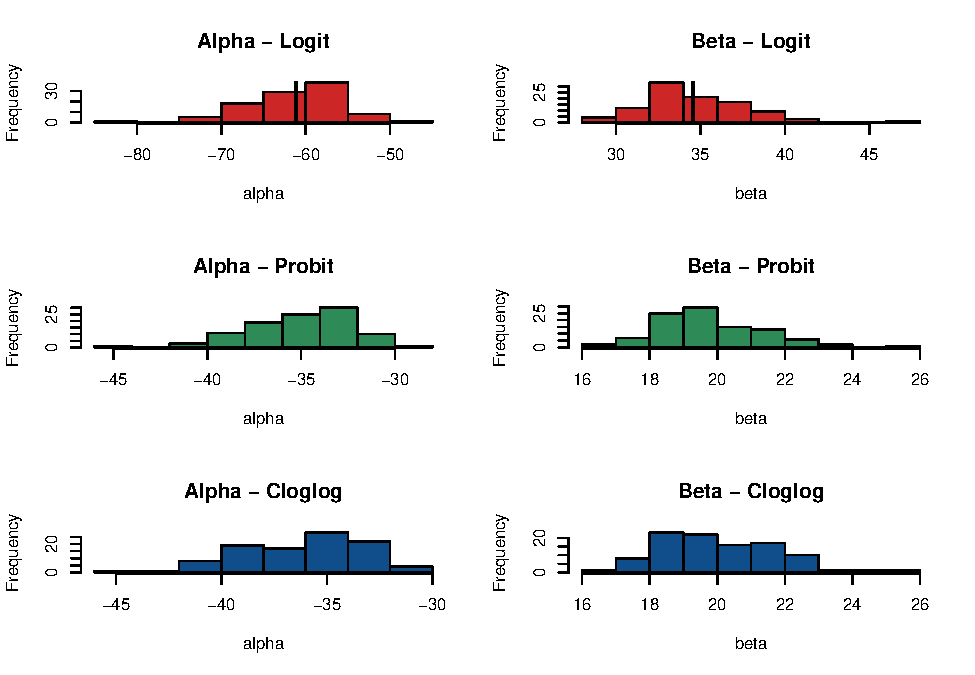
\includegraphics{FinalProject-SDSII_files/figure-latex/unnamed-chunk-36-1.pdf}

\begin{Shaded}
\begin{Highlighting}[]
\KeywordTok{kable}\NormalTok{(}\KeywordTok{summary}\NormalTok{(res[, }\KeywordTok{c}\NormalTok{(}\StringTok{'logit_DIC'}\NormalTok{,}\StringTok{'probit_DIC'}\NormalTok{, }\StringTok{'cloglog_DIC'}\NormalTok{)]), }\StringTok{'latex'}\NormalTok{, }\DataTypeTok{booktabs =}\NormalTok{ T) }\OperatorTok
\StringTok{  }\KeywordTok{kable_styling}\NormalTok{(}\DataTypeTok{latex_options =} \KeywordTok{c}\NormalTok{(}\StringTok{"striped"}\NormalTok{, }\StringTok{"hold_position"}\NormalTok{))}
\end{Highlighting}
\end{Shaded}

\begin{table}[!h]
\centering
\begin{tabular}{llll}
\toprule
  &   logit\_DIC &   probit\_DIC &  cloglog\_DIC\\
\midrule
\rowcolor{gray!6}   & Min.   : 97.02 & Min.   :31.91 & Min.   :30.12\\
 & 1st Qu.:116.31 & 1st Qu.:35.05 & 1st Qu.:39.45\\
\rowcolor{gray!6}   & Median :124.18 & Median :36.96 & Median :43.84\\
 & Mean   :125.06 & Mean   :38.18 & Mean   :45.62\\
\rowcolor{gray!6}   & 3rd Qu.:134.47 & 3rd Qu.:41.13 & 3rd Qu.:50.73\\
\addlinespace
 & Max.   :159.03 & Max.   :53.22 & Max.   :69.83\\
\bottomrule
\end{tabular}
\end{table}

\begin{Shaded}
\begin{Highlighting}[]
\NormalTok{true_alpha =}\StringTok{ }\KeywordTok{rep}\NormalTok{(a, }\DecValTok{100}\NormalTok{) }
\NormalTok{true_beta =}\StringTok{ }\KeywordTok{rep}\NormalTok{(b, }\DecValTok{100}\NormalTok{)}
\NormalTok{rmse_logit =}\StringTok{ }\KeywordTok{c}\NormalTok{(}\KeywordTok{RMSE}\NormalTok{(res[,}\StringTok{'logit_alpha'}\NormalTok{],true_alpha),}\KeywordTok{RMSE}\NormalTok{(res[,}\StringTok{'logit_beta'}\NormalTok{],true_beta))}
\NormalTok{rmse_probit =}\StringTok{ }\KeywordTok{c}\NormalTok{(}\KeywordTok{RMSE}\NormalTok{(res[,}\StringTok{'probit_alpha'}\NormalTok{],true_alpha),}\KeywordTok{RMSE}\NormalTok{(res[,}\StringTok{'probit_beta'}\NormalTok{],true_beta))}
\NormalTok{rmse_cloglog =}\StringTok{ }\KeywordTok{c}\NormalTok{(}\KeywordTok{RMSE}\NormalTok{(res[,}\StringTok{'cloglog_alpha'}\NormalTok{],true_alpha),}\KeywordTok{RMSE}\NormalTok{(res[,}\StringTok{'cloglog_beta'}\NormalTok{],true_beta))}
\NormalTok{toprint =}\StringTok{ }\KeywordTok{as.data.frame}\NormalTok{(}\KeywordTok{cbind}\NormalTok{(rmse_logit, rmse_probit, rmse_cloglog))}
\KeywordTok{names}\NormalTok{(toprint) <-}\StringTok{ }\KeywordTok{c}\NormalTok{(}\StringTok{'Logistic'}\NormalTok{, }\StringTok{'Probit'}\NormalTok{, }\StringTok{'Extreme values'}\NormalTok{)}
\KeywordTok{row.names}\NormalTok{(toprint) <-}\StringTok{ }\KeywordTok{c}\NormalTok{(}\StringTok{'Alpha'}\NormalTok{, }\StringTok{'Beta'}\NormalTok{)}

\KeywordTok{kable}\NormalTok{(toprint, }\StringTok{"latex"}\NormalTok{, }\DataTypeTok{booktabs =}\NormalTok{ T) }\OperatorTok
\StringTok{  }\KeywordTok{kable_styling}\NormalTok{(}\DataTypeTok{latex_options =}\KeywordTok{c}\NormalTok{(}\StringTok{"striped"}\NormalTok{, }\StringTok{"hold_position"}\NormalTok{))}
\end{Highlighting}
\end{Shaded}

\begin{table}[!h]
\centering
\begin{tabular}{lrrr}
\toprule
  & Logistic & Probit & Extreme values\\
\midrule
\rowcolor{gray!6}  Alpha & 5.410247 & 26.34490 & 25.34154\\
Beta & 3.036789 & 14.88004 & 14.59721\\
\bottomrule
\end{tabular}
\end{table}

Let's have a look also at the probit and extreme values models, before
proceeding with the commentary.\\
The next model then is the probit:

\begin{Shaded}
\begin{Highlighting}[]
\NormalTok{n_data =}\StringTok{ }\DecValTok{100}
\NormalTok{res <-}\StringTok{ }\KeywordTok{matrix}\NormalTok{(}\KeywordTok{rep}\NormalTok{(}\OtherTok{NA}\NormalTok{,n_data}\OperatorTok{*}\DecValTok{3}\OperatorTok{*}\DecValTok{3}\NormalTok{), }\DataTypeTok{nrow =}\NormalTok{ n_data, }\DataTypeTok{ncol =} \DecValTok{9}\NormalTok{)}
\KeywordTok{colnames}\NormalTok{(res) <-}\StringTok{ }\KeywordTok{c}\NormalTok{(}\StringTok{'logit_alpha'}\NormalTok{,}\StringTok{'logit_beta'}\NormalTok{,}\StringTok{'logit_DIC'}\NormalTok{,}
                   \StringTok{'probit_alpha'}\NormalTok{,}\StringTok{'probit_beta'}\NormalTok{,}\StringTok{'probit_DIC'}\NormalTok{,}
                   \StringTok{'cloglog_alpha'}\NormalTok{,}\StringTok{'cloglog_beta'}\NormalTok{,}\StringTok{'cloglog_DIC'}\NormalTok{)}
\NormalTok{a <-}\StringTok{ }\NormalTok{probit_res}\OperatorTok{$}\NormalTok{BUGSoutput}\OperatorTok{$}\NormalTok{mean}\OperatorTok{$}\NormalTok{alpha}
\NormalTok{b <-}\StringTok{ }\NormalTok{probit_res}\OperatorTok{$}\NormalTok{BUGSoutput}\OperatorTok{$}\NormalTok{mean}\OperatorTok{$}\NormalTok{beta}

\ControlFlowTok{for}\NormalTok{(i }\ControlFlowTok{in} \DecValTok{1}\OperatorTok{:}\NormalTok{n_data)\{}

\NormalTok{  y_new =}\StringTok{ }\KeywordTok{rbinom}\NormalTok{(}\KeywordTok{length}\NormalTok{(data}\OperatorTok{$}\NormalTok{n), data}\OperatorTok{$}\NormalTok{n, }\KeywordTok{pnorm}\NormalTok{(alpha }\OperatorTok{+}\StringTok{ }\NormalTok{(beta }\OperatorTok{*}\StringTok{ }\NormalTok{data}\OperatorTok{$}\NormalTok{x), }\DataTypeTok{mean =} \DecValTok{0}\NormalTok{, }\DataTypeTok{sd =} \DecValTok{1}\NormalTok{, }\DataTypeTok{lower.tail =} \OtherTok{TRUE}\NormalTok{))}
                

\NormalTok{  data.list=}\StringTok{ }\KeywordTok{list}\NormalTok{(}\DataTypeTok{r =}\NormalTok{ y_new,}
                \DataTypeTok{n =}\NormalTok{ data}\OperatorTok{$}\NormalTok{n,}
                \DataTypeTok{x =}\NormalTok{ data}\OperatorTok{$}\NormalTok{x,}
                \DataTypeTok{tau_alpha =}\NormalTok{ tau_alpha,}
                \DataTypeTok{tau_beta =}\NormalTok{ tau_beta,}
                \DataTypeTok{N =} \DecValTok{8}\NormalTok{)}
  
\NormalTok{  mcmc_res =}\StringTok{ }\KeywordTok{jags}\NormalTok{( }\DataTypeTok{model.file =} \KeywordTok{textConnection}\NormalTok{(model_}\DecValTok{1}\NormalTok{),}
                  \DataTypeTok{data =}\NormalTok{ data.list, }
                  \DataTypeTok{n.chains =} \DecValTok{3}\NormalTok{, }
                  \DataTypeTok{n.iter =} \DecValTok{11000}\NormalTok{, }
                  \DataTypeTok{n.burnin =} \DecValTok{1000}\NormalTok{,}
                  \DataTypeTok{inits =}\NormalTok{ init.list.nod, }
                  \DataTypeTok{parameters.to.save =} \KeywordTok{c}\NormalTok{(}\StringTok{"alpha"}\NormalTok{,}\StringTok{"alpha.star"}\NormalTok{,}\StringTok{"beta"}\NormalTok{))}
  
\NormalTok{  res[i, }\StringTok{'logit_alpha'}\NormalTok{] =}\StringTok{ }\NormalTok{mcmc_res}\OperatorTok{$}\NormalTok{BUGSoutput}\OperatorTok{$}\NormalTok{mean}\OperatorTok{$}\NormalTok{alpha}
\NormalTok{  res[i, }\StringTok{'logit_beta'}\NormalTok{] =}\StringTok{ }\NormalTok{mcmc_res}\OperatorTok{$}\NormalTok{BUGSoutput}\OperatorTok{$}\NormalTok{mean}\OperatorTok{$}\NormalTok{beta}
\NormalTok{  res[i, }\StringTok{'logit_DIC'}\NormalTok{] =}\StringTok{ }\NormalTok{mcmc_res}\OperatorTok{$}\NormalTok{BUGSoutput}\OperatorTok{$}\NormalTok{DIC}
  
\NormalTok{  mcmc_res =}\StringTok{ }\KeywordTok{jags}\NormalTok{( }\DataTypeTok{model.file =} \KeywordTok{textConnection}\NormalTok{(model_}\DecValTok{2}\NormalTok{),}
                  \DataTypeTok{data =}\NormalTok{ data.list, }
                  \DataTypeTok{n.chains =} \DecValTok{3}\NormalTok{, }
                  \DataTypeTok{n.iter =} \DecValTok{11000}\NormalTok{, }
                  \DataTypeTok{n.burnin =} \DecValTok{1000}\NormalTok{,}
                  \DataTypeTok{inits =}\NormalTok{ init.list.nod, }
                  \DataTypeTok{parameters.to.save =} \KeywordTok{c}\NormalTok{(}\StringTok{"alpha"}\NormalTok{,}\StringTok{"alpha.star"}\NormalTok{,}\StringTok{"beta"}\NormalTok{))}
  
\NormalTok{  res[i, }\StringTok{'probit_alpha'}\NormalTok{] =}\StringTok{ }\NormalTok{mcmc_res}\OperatorTok{$}\NormalTok{BUGSoutput}\OperatorTok{$}\NormalTok{mean}\OperatorTok{$}\NormalTok{alpha}
\NormalTok{  res[i, }\StringTok{'probit_beta'}\NormalTok{] =}\StringTok{ }\NormalTok{mcmc_res}\OperatorTok{$}\NormalTok{BUGSoutput}\OperatorTok{$}\NormalTok{mean}\OperatorTok{$}\NormalTok{beta}
\NormalTok{  res[i, }\StringTok{'probit_DIC'}\NormalTok{] =}\StringTok{ }\NormalTok{mcmc_res}\OperatorTok{$}\NormalTok{BUGSoutput}\OperatorTok{$}\NormalTok{DIC}
  
\NormalTok{    mcmc_res =}\StringTok{ }\KeywordTok{jags}\NormalTok{( }\DataTypeTok{model.file =} \KeywordTok{textConnection}\NormalTok{(model_}\DecValTok{3}\NormalTok{),}
                  \DataTypeTok{data =}\NormalTok{ data.list, }
                  \DataTypeTok{n.chains =} \DecValTok{3}\NormalTok{, }
                  \DataTypeTok{n.iter =} \DecValTok{11000}\NormalTok{, }
                  \DataTypeTok{n.burnin =} \DecValTok{1000}\NormalTok{,}
                  \DataTypeTok{inits =}\NormalTok{ init.list.nod, }
                  \DataTypeTok{parameters.to.save =} \KeywordTok{c}\NormalTok{(}\StringTok{"alpha"}\NormalTok{,}\StringTok{"alpha.star"}\NormalTok{,}\StringTok{"beta"}\NormalTok{))}
  
\NormalTok{  res[i, }\StringTok{'cloglog_alpha'}\NormalTok{] =}\StringTok{ }\NormalTok{mcmc_res}\OperatorTok{$}\NormalTok{BUGSoutput}\OperatorTok{$}\NormalTok{mean}\OperatorTok{$}\NormalTok{alpha}
\NormalTok{  res[i, }\StringTok{'cloglog_beta'}\NormalTok{] =}\StringTok{ }\NormalTok{mcmc_res}\OperatorTok{$}\NormalTok{BUGSoutput}\OperatorTok{$}\NormalTok{mean}\OperatorTok{$}\NormalTok{beta}
\NormalTok{  res[i, }\StringTok{'cloglog_DIC'}\NormalTok{] =}\StringTok{ }\NormalTok{mcmc_res}\OperatorTok{$}\NormalTok{BUGSoutput}\OperatorTok{$}\NormalTok{DIC}
\NormalTok{\}}
\end{Highlighting}
\end{Shaded}

\begin{Shaded}
\begin{Highlighting}[]
\KeywordTok{par}\NormalTok{(}\DataTypeTok{mfrow =} \KeywordTok{c}\NormalTok{(}\DecValTok{3}\NormalTok{,}\DecValTok{2}\NormalTok{))}
\KeywordTok{hist}\NormalTok{(res[, }\StringTok{'logit_alpha'}\NormalTok{], }\DataTypeTok{main =} \StringTok{"Alpha - Logit"}\NormalTok{, }\DataTypeTok{col =} \StringTok{"firebrick3"}\NormalTok{, }\DataTypeTok{xlab =} \StringTok{'alpha'}\NormalTok{) }
\KeywordTok{abline}\NormalTok{(}\DataTypeTok{v =}\NormalTok{ a, }\DataTypeTok{lwd =} \DecValTok{2}\NormalTok{)}
\KeywordTok{hist}\NormalTok{(res[, }\StringTok{'logit_beta'}\NormalTok{], }\DataTypeTok{main =} \StringTok{"Beta - Logit"}\NormalTok{, }\DataTypeTok{col =} \StringTok{"firebrick3"}\NormalTok{, }\DataTypeTok{xlab =} \StringTok{'beta'}\NormalTok{) }
\KeywordTok{abline}\NormalTok{(}\DataTypeTok{v =}\NormalTok{ b, }\DataTypeTok{lwd =} \DecValTok{2}\NormalTok{)}

\KeywordTok{hist}\NormalTok{(res[, }\StringTok{'probit_alpha'}\NormalTok{], }\DataTypeTok{main =} \StringTok{"Alpha - Probit"}\NormalTok{, }\DataTypeTok{col =} \StringTok{"seagreen4"}\NormalTok{, }\DataTypeTok{xlab =} \StringTok{'alpha'}\NormalTok{) }
\KeywordTok{abline}\NormalTok{(}\DataTypeTok{v =}\NormalTok{ a, }\DataTypeTok{lwd =} \DecValTok{2}\NormalTok{)}
\KeywordTok{hist}\NormalTok{(res[, }\StringTok{'probit_beta'}\NormalTok{], }\DataTypeTok{main =} \StringTok{"Beta - Probit"}\NormalTok{, }\DataTypeTok{col =} \StringTok{"seagreen4"}\NormalTok{, }\DataTypeTok{xlab =} \StringTok{'beta'}\NormalTok{) }
\KeywordTok{abline}\NormalTok{(}\DataTypeTok{v =}\NormalTok{ b, }\DataTypeTok{lwd =} \DecValTok{2}\NormalTok{)}

\KeywordTok{hist}\NormalTok{(res[, }\StringTok{'cloglog_alpha'}\NormalTok{], }\DataTypeTok{main =} \StringTok{"Alpha - Cloglog"}\NormalTok{, }\DataTypeTok{col =} \StringTok{"dodgerblue4"}\NormalTok{, }\DataTypeTok{xlab =} \StringTok{'alpha'}\NormalTok{) }
\KeywordTok{abline}\NormalTok{(}\DataTypeTok{v =}\NormalTok{ a, }\DataTypeTok{lwd =} \DecValTok{2}\NormalTok{)}
\KeywordTok{hist}\NormalTok{(res[, }\StringTok{'cloglog_beta'}\NormalTok{], }\DataTypeTok{main =} \StringTok{"Beta - Cloglog"}\NormalTok{, }\DataTypeTok{col =} \StringTok{"dodgerblue4"}\NormalTok{, }\DataTypeTok{xlab =} \StringTok{'beta'}\NormalTok{) }
\KeywordTok{abline}\NormalTok{(}\DataTypeTok{v =}\NormalTok{ b, }\DataTypeTok{lwd =} \DecValTok{2}\NormalTok{)}
\end{Highlighting}
\end{Shaded}

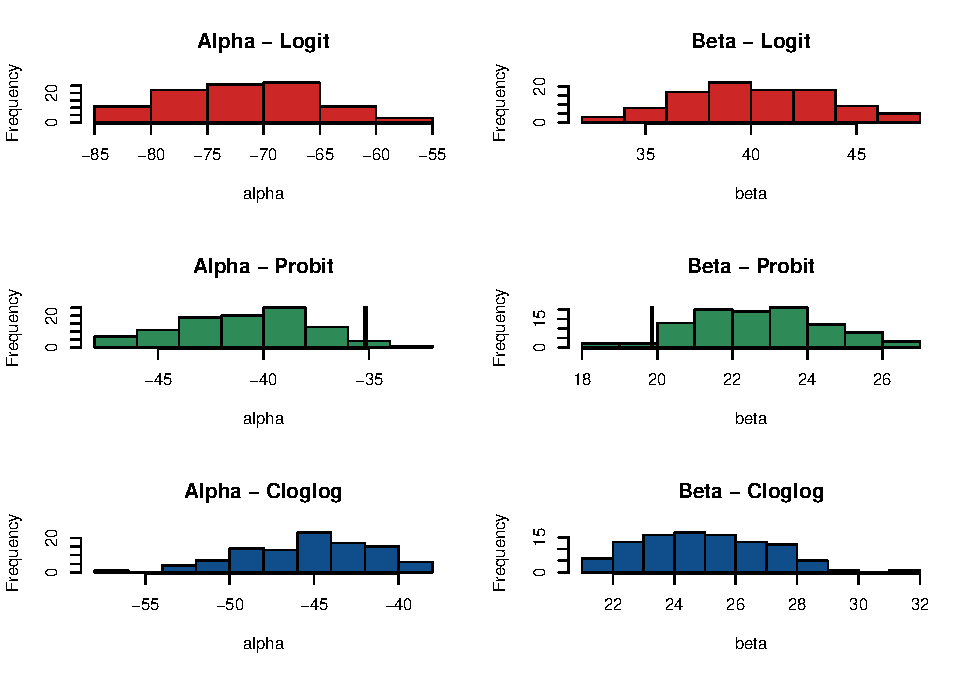
\includegraphics{FinalProject-SDSII_files/figure-latex/unnamed-chunk-40-1.pdf}

\begin{Shaded}
\begin{Highlighting}[]
\KeywordTok{kable}\NormalTok{(}\KeywordTok{summary}\NormalTok{(res[, }\KeywordTok{c}\NormalTok{(}\StringTok{'logit_DIC'}\NormalTok{,}\StringTok{'probit_DIC'}\NormalTok{, }\StringTok{'cloglog_DIC'}\NormalTok{)]), }\StringTok{'latex'}\NormalTok{, }\DataTypeTok{booktabs =}\NormalTok{ T) }\OperatorTok
\StringTok{  }\KeywordTok{kable_styling}\NormalTok{(}\DataTypeTok{latex_options =} \KeywordTok{c}\NormalTok{(}\StringTok{"striped"}\NormalTok{, }\StringTok{"hold_position"}\NormalTok{))}
\end{Highlighting}
\end{Shaded}

\begin{table}[!h]
\centering
\begin{tabular}{llll}
\toprule
  &   logit\_DIC &   probit\_DIC &  cloglog\_DIC\\
\midrule
\rowcolor{gray!6}   & Min.   :157.6 & Min.   :30.19 & Min.   :31.91\\
 & 1st Qu.:187.3 & 1st Qu.:34.55 & 1st Qu.:39.38\\
\rowcolor{gray!6}   & Median :200.3 & Median :36.19 & Median :43.62\\
 & Mean   :200.4 & Mean   :36.57 & Mean   :43.47\\
\rowcolor{gray!6}   & 3rd Qu.:214.2 & 3rd Qu.:38.62 & 3rd Qu.:46.83\\
\addlinespace
 & Max.   :241.8 & Max.   :46.39 & Max.   :61.80\\
\bottomrule
\end{tabular}
\end{table}

\begin{Shaded}
\begin{Highlighting}[]
\NormalTok{true_alpha =}\StringTok{ }\KeywordTok{rep}\NormalTok{(a, }\DecValTok{100}\NormalTok{) }
\NormalTok{true_beta =}\StringTok{ }\KeywordTok{rep}\NormalTok{(b, }\DecValTok{100}\NormalTok{)}
\NormalTok{rmse_logit =}\StringTok{ }\KeywordTok{c}\NormalTok{(}\KeywordTok{RMSE}\NormalTok{(res[,}\StringTok{'logit_alpha'}\NormalTok{],true_alpha),}\KeywordTok{RMSE}\NormalTok{(res[,}\StringTok{'logit_beta'}\NormalTok{],true_beta))}
\NormalTok{rmse_probit =}\StringTok{ }\KeywordTok{c}\NormalTok{(}\KeywordTok{RMSE}\NormalTok{(res[,}\StringTok{'probit_alpha'}\NormalTok{],true_alpha),}\KeywordTok{RMSE}\NormalTok{(res[,}\StringTok{'probit_beta'}\NormalTok{],true_beta))}
\NormalTok{rmse_cloglog =}\StringTok{ }\KeywordTok{c}\NormalTok{(}\KeywordTok{RMSE}\NormalTok{(res[,}\StringTok{'cloglog_alpha'}\NormalTok{],true_alpha),}\KeywordTok{RMSE}\NormalTok{(res[,}\StringTok{'cloglog_beta'}\NormalTok{],true_beta))}
\NormalTok{toprint =}\StringTok{ }\KeywordTok{as.data.frame}\NormalTok{(}\KeywordTok{cbind}\NormalTok{(rmse_logit, rmse_probit, rmse_cloglog))}
\KeywordTok{names}\NormalTok{(toprint) <-}\StringTok{ }\KeywordTok{c}\NormalTok{(}\StringTok{'Logistic'}\NormalTok{, }\StringTok{'Probit'}\NormalTok{, }\StringTok{'Extreme values'}\NormalTok{)}
\KeywordTok{row.names}\NormalTok{(toprint) <-}\StringTok{ }\KeywordTok{c}\NormalTok{(}\StringTok{'Alpha'}\NormalTok{, }\StringTok{'Beta'}\NormalTok{)}

\KeywordTok{kable}\NormalTok{(toprint, }\StringTok{"latex"}\NormalTok{, }\DataTypeTok{booktabs =}\NormalTok{ T) }\OperatorTok
\StringTok{  }\KeywordTok{kable_styling}\NormalTok{(}\DataTypeTok{latex_options =}\KeywordTok{c}\NormalTok{(}\StringTok{"striped"}\NormalTok{, }\StringTok{"hold_position"}\NormalTok{))}
\end{Highlighting}
\end{Shaded}

\begin{table}[!h]
\centering
\begin{tabular}{lrrr}
\toprule
  & Logistic & Probit & Extreme values\\
\midrule
\rowcolor{gray!6}  Alpha & 37.37204 & 6.472876 & 10.910925\\
Beta & 20.53763 & 3.365092 & 5.521215\\
\bottomrule
\end{tabular}
\end{table}

And finally we have a look also at the extreme values results:

\begin{Shaded}
\begin{Highlighting}[]
\NormalTok{n_data =}\StringTok{ }\DecValTok{100}
\NormalTok{res <-}\StringTok{ }\KeywordTok{matrix}\NormalTok{(}\KeywordTok{rep}\NormalTok{(}\OtherTok{NA}\NormalTok{,n_data}\OperatorTok{*}\DecValTok{3}\OperatorTok{*}\DecValTok{3}\NormalTok{), }\DataTypeTok{nrow =}\NormalTok{ n_data, }\DataTypeTok{ncol =} \DecValTok{9}\NormalTok{)}
\KeywordTok{colnames}\NormalTok{(res) <-}\StringTok{ }\KeywordTok{c}\NormalTok{(}\StringTok{'logit_alpha'}\NormalTok{,}\StringTok{'logit_beta'}\NormalTok{,}\StringTok{'logit_DIC'}\NormalTok{,}
                   \StringTok{'probit_alpha'}\NormalTok{,}\StringTok{'probit_beta'}\NormalTok{,}\StringTok{'probit_DIC'}\NormalTok{,}
                   \StringTok{'cloglog_alpha'}\NormalTok{,}\StringTok{'cloglog_beta'}\NormalTok{,}\StringTok{'cloglog_DIC'}\NormalTok{)}
\NormalTok{a <-}\StringTok{ }\NormalTok{cloglog_res}\OperatorTok{$}\NormalTok{BUGSoutput}\OperatorTok{$}\NormalTok{mean}\OperatorTok{$}\NormalTok{alpha}
\NormalTok{b <-}\StringTok{ }\NormalTok{cloglog_res}\OperatorTok{$}\NormalTok{BUGSoutput}\OperatorTok{$}\NormalTok{mean}\OperatorTok{$}\NormalTok{beta}

\ControlFlowTok{for}\NormalTok{(i }\ControlFlowTok{in} \DecValTok{1}\OperatorTok{:}\NormalTok{n_data)\{}

\NormalTok{  y_new =}\StringTok{ }\KeywordTok{rbinom}\NormalTok{(}\KeywordTok{length}\NormalTok{(data}\OperatorTok{$}\NormalTok{n), data}\OperatorTok{$}\NormalTok{n, }\KeywordTok{cloglog}\NormalTok{(data}\OperatorTok{$}\NormalTok{x, a, b))}
  
\NormalTok{  data.list=}\StringTok{ }\KeywordTok{list}\NormalTok{(}\DataTypeTok{r =}\NormalTok{ y_new,}
                \DataTypeTok{n =}\NormalTok{ data}\OperatorTok{$}\NormalTok{n,}
                \DataTypeTok{x =}\NormalTok{ data}\OperatorTok{$}\NormalTok{x,}
                \DataTypeTok{tau_alpha =}\NormalTok{ tau_alpha,}
                \DataTypeTok{tau_beta =}\NormalTok{ tau_beta,}
                \DataTypeTok{N =} \DecValTok{8}\NormalTok{)}
  
\NormalTok{  mcmc_res =}\StringTok{ }\KeywordTok{jags}\NormalTok{( }\DataTypeTok{model.file =} \KeywordTok{textConnection}\NormalTok{(model_}\DecValTok{1}\NormalTok{),}
                  \DataTypeTok{data =}\NormalTok{ data.list, }
                  \DataTypeTok{n.chains =} \DecValTok{3}\NormalTok{, }
                  \DataTypeTok{n.iter =} \DecValTok{11000}\NormalTok{, }
                  \DataTypeTok{n.burnin =} \DecValTok{1000}\NormalTok{,}
                  \DataTypeTok{inits =}\NormalTok{ init.list.nod, }
                  \DataTypeTok{parameters.to.save =} \KeywordTok{c}\NormalTok{(}\StringTok{"alpha"}\NormalTok{,}\StringTok{"alpha.star"}\NormalTok{,}\StringTok{"beta"}\NormalTok{))}
  
\NormalTok{  res[i, }\StringTok{'logit_alpha'}\NormalTok{] =}\StringTok{ }\NormalTok{mcmc_res}\OperatorTok{$}\NormalTok{BUGSoutput}\OperatorTok{$}\NormalTok{mean}\OperatorTok{$}\NormalTok{alpha}
\NormalTok{  res[i, }\StringTok{'logit_beta'}\NormalTok{] =}\StringTok{ }\NormalTok{mcmc_res}\OperatorTok{$}\NormalTok{BUGSoutput}\OperatorTok{$}\NormalTok{mean}\OperatorTok{$}\NormalTok{beta}
\NormalTok{  res[i, }\StringTok{'logit_DIC'}\NormalTok{] =}\StringTok{ }\NormalTok{mcmc_res}\OperatorTok{$}\NormalTok{BUGSoutput}\OperatorTok{$}\NormalTok{DIC}
  
\NormalTok{  mcmc_res =}\StringTok{ }\KeywordTok{jags}\NormalTok{( }\DataTypeTok{model.file =} \KeywordTok{textConnection}\NormalTok{(model_}\DecValTok{2}\NormalTok{),}
                  \DataTypeTok{data =}\NormalTok{ data.list, }
                  \DataTypeTok{n.chains =} \DecValTok{3}\NormalTok{, }
                  \DataTypeTok{n.iter =} \DecValTok{11000}\NormalTok{, }
                  \DataTypeTok{n.burnin =} \DecValTok{1000}\NormalTok{,}
                  \DataTypeTok{inits =}\NormalTok{ init.list.nod, }
                  \DataTypeTok{parameters.to.save =} \KeywordTok{c}\NormalTok{(}\StringTok{"alpha"}\NormalTok{,}\StringTok{"alpha.star"}\NormalTok{,}\StringTok{"beta"}\NormalTok{))}
  
\NormalTok{  res[i, }\StringTok{'probit_alpha'}\NormalTok{] =}\StringTok{ }\NormalTok{mcmc_res}\OperatorTok{$}\NormalTok{BUGSoutput}\OperatorTok{$}\NormalTok{mean}\OperatorTok{$}\NormalTok{alpha}
\NormalTok{  res[i, }\StringTok{'probit_beta'}\NormalTok{] =}\StringTok{ }\NormalTok{mcmc_res}\OperatorTok{$}\NormalTok{BUGSoutput}\OperatorTok{$}\NormalTok{mean}\OperatorTok{$}\NormalTok{beta}
\NormalTok{  res[i, }\StringTok{'probit_DIC'}\NormalTok{] =}\StringTok{ }\NormalTok{mcmc_res}\OperatorTok{$}\NormalTok{BUGSoutput}\OperatorTok{$}\NormalTok{DIC}
  
\NormalTok{    mcmc_res =}\StringTok{ }\KeywordTok{jags}\NormalTok{( }\DataTypeTok{model.file =} \KeywordTok{textConnection}\NormalTok{(model_}\DecValTok{3}\NormalTok{),}
                  \DataTypeTok{data =}\NormalTok{ data.list, }
                  \DataTypeTok{n.chains =} \DecValTok{3}\NormalTok{, }
                  \DataTypeTok{n.iter =} \DecValTok{11000}\NormalTok{, }
                  \DataTypeTok{n.burnin =} \DecValTok{1000}\NormalTok{,}
                  \DataTypeTok{inits =}\NormalTok{ init.list.nod, }
                  \DataTypeTok{parameters.to.save =} \KeywordTok{c}\NormalTok{(}\StringTok{"alpha"}\NormalTok{,}\StringTok{"alpha.star"}\NormalTok{,}\StringTok{"beta"}\NormalTok{))}
  
\NormalTok{  res[i, }\StringTok{'cloglog_alpha'}\NormalTok{] =}\StringTok{ }\NormalTok{mcmc_res}\OperatorTok{$}\NormalTok{BUGSoutput}\OperatorTok{$}\NormalTok{mean}\OperatorTok{$}\NormalTok{alpha}
\NormalTok{  res[i, }\StringTok{'cloglog_beta'}\NormalTok{] =}\StringTok{ }\NormalTok{mcmc_res}\OperatorTok{$}\NormalTok{BUGSoutput}\OperatorTok{$}\NormalTok{mean}\OperatorTok{$}\NormalTok{beta}
\NormalTok{  res[i, }\StringTok{'cloglog_DIC'}\NormalTok{] =}\StringTok{ }\NormalTok{mcmc_res}\OperatorTok{$}\NormalTok{BUGSoutput}\OperatorTok{$}\NormalTok{DIC}
\NormalTok{\}}
\end{Highlighting}
\end{Shaded}

\begin{Shaded}
\begin{Highlighting}[]
\KeywordTok{par}\NormalTok{(}\DataTypeTok{mfrow =} \KeywordTok{c}\NormalTok{(}\DecValTok{3}\NormalTok{,}\DecValTok{2}\NormalTok{))}
\KeywordTok{hist}\NormalTok{(res[, }\StringTok{'logit_alpha'}\NormalTok{], }\DataTypeTok{main =} \StringTok{"Alpha - Logit"}\NormalTok{, }\DataTypeTok{col =} \StringTok{"firebrick3"}\NormalTok{, }\DataTypeTok{xlab =} \StringTok{'alpha'}\NormalTok{) }
\KeywordTok{abline}\NormalTok{(}\DataTypeTok{v =}\NormalTok{ a, }\DataTypeTok{lwd =} \DecValTok{2}\NormalTok{)}
\KeywordTok{hist}\NormalTok{(res[, }\StringTok{'logit_beta'}\NormalTok{], }\DataTypeTok{main =} \StringTok{"Beta - Logit"}\NormalTok{, }\DataTypeTok{col =} \StringTok{"firebrick3"}\NormalTok{, }\DataTypeTok{xlab =} \StringTok{'beta'}\NormalTok{) }
\KeywordTok{abline}\NormalTok{(}\DataTypeTok{v =}\NormalTok{ b, }\DataTypeTok{lwd =} \DecValTok{2}\NormalTok{)}

\KeywordTok{hist}\NormalTok{(res[, }\StringTok{'probit_alpha'}\NormalTok{], }\DataTypeTok{main =} \StringTok{"Alpha - Probit"}\NormalTok{, }\DataTypeTok{col =} \StringTok{"seagreen4"}\NormalTok{, }\DataTypeTok{xlab =} \StringTok{'alpha'}\NormalTok{) }
\KeywordTok{abline}\NormalTok{(}\DataTypeTok{v =}\NormalTok{ a, }\DataTypeTok{lwd =} \DecValTok{2}\NormalTok{)}
\KeywordTok{hist}\NormalTok{(res[, }\StringTok{'probit_beta'}\NormalTok{], }\DataTypeTok{main =} \StringTok{"Beta - Probit"}\NormalTok{, }\DataTypeTok{col =} \StringTok{"seagreen4"}\NormalTok{, }\DataTypeTok{xlab =} \StringTok{'beta'}\NormalTok{) }
\KeywordTok{abline}\NormalTok{(}\DataTypeTok{v =}\NormalTok{ b, }\DataTypeTok{lwd =} \DecValTok{2}\NormalTok{)}

\KeywordTok{hist}\NormalTok{(res[, }\StringTok{'cloglog_alpha'}\NormalTok{], }\DataTypeTok{main =} \StringTok{"Alpha - Cloglog"}\NormalTok{, }\DataTypeTok{col =} \StringTok{"dodgerblue4"}\NormalTok{, }\DataTypeTok{xlab =} \StringTok{'alpha'}\NormalTok{) }
\KeywordTok{abline}\NormalTok{(}\DataTypeTok{v =}\NormalTok{ a, }\DataTypeTok{lwd =} \DecValTok{2}\NormalTok{)}
\KeywordTok{hist}\NormalTok{(res[, }\StringTok{'cloglog_beta'}\NormalTok{], }\DataTypeTok{main =} \StringTok{"Beta - Cloglog"}\NormalTok{, }\DataTypeTok{col =} \StringTok{"dodgerblue4"}\NormalTok{, }\DataTypeTok{xlab =} \StringTok{'beta'}\NormalTok{) }
\KeywordTok{abline}\NormalTok{(}\DataTypeTok{v =}\NormalTok{ b, }\DataTypeTok{lwd =} \DecValTok{2}\NormalTok{)}
\end{Highlighting}
\end{Shaded}

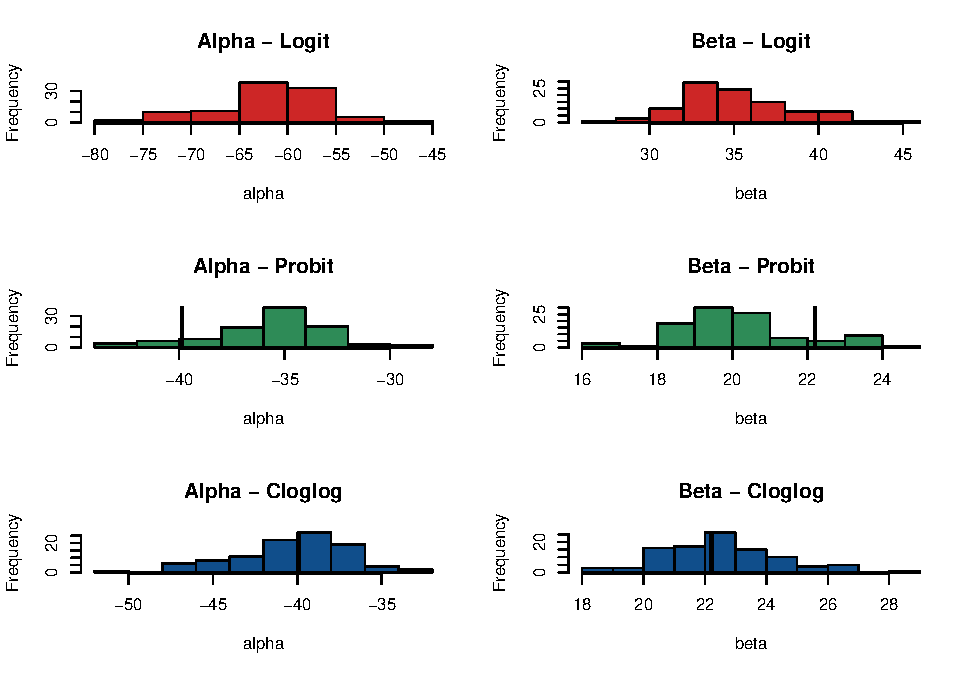
\includegraphics{FinalProject-SDSII_files/figure-latex/unnamed-chunk-44-1.pdf}

\begin{Shaded}
\begin{Highlighting}[]
\KeywordTok{kable}\NormalTok{(}\KeywordTok{summary}\NormalTok{(res[, }\KeywordTok{c}\NormalTok{(}\StringTok{'logit_DIC'}\NormalTok{,}\StringTok{'probit_DIC'}\NormalTok{, }\StringTok{'cloglog_DIC'}\NormalTok{)]), }\StringTok{'latex'}\NormalTok{, }\DataTypeTok{booktabs =}\NormalTok{ T) }\OperatorTok
\StringTok{  }\KeywordTok{kable_styling}\NormalTok{(}\DataTypeTok{latex_options =} \KeywordTok{c}\NormalTok{(}\StringTok{"striped"}\NormalTok{, }\StringTok{"hold_position"}\NormalTok{))}
\end{Highlighting}
\end{Shaded}

\begin{table}[!h]
\centering
\begin{tabular}{llll}
\toprule
  &   logit\_DIC &   probit\_DIC &  cloglog\_DIC\\
\midrule
\rowcolor{gray!6}   & Min.   :105.3 & Min.   :32.20 & Min.   :29.55\\
 & 1st Qu.:120.7 & 1st Qu.:37.32 & 1st Qu.:32.51\\
\rowcolor{gray!6}   & Median :128.2 & Median :39.81 & Median :34.86\\
 & Mean   :128.7 & Mean   :40.37 & Mean   :35.18\\
\rowcolor{gray!6}   & 3rd Qu.:135.7 & 3rd Qu.:42.72 & 3rd Qu.:37.43\\
\addlinespace
 & Max.   :174.1 & Max.   :54.36 & Max.   :47.09\\
\bottomrule
\end{tabular}
\end{table}

\begin{Shaded}
\begin{Highlighting}[]
\NormalTok{true_alpha =}\StringTok{ }\KeywordTok{rep}\NormalTok{(a, }\DecValTok{100}\NormalTok{) }
\NormalTok{true_beta =}\StringTok{ }\KeywordTok{rep}\NormalTok{(b, }\DecValTok{100}\NormalTok{)}
\NormalTok{rmse_logit =}\StringTok{ }\KeywordTok{c}\NormalTok{(}\KeywordTok{RMSE}\NormalTok{(res[,}\StringTok{'logit_alpha'}\NormalTok{],true_alpha),}\KeywordTok{RMSE}\NormalTok{(res[,}\StringTok{'logit_beta'}\NormalTok{],true_beta))}
\NormalTok{rmse_probit =}\StringTok{ }\KeywordTok{c}\NormalTok{(}\KeywordTok{RMSE}\NormalTok{(res[,}\StringTok{'probit_alpha'}\NormalTok{],true_alpha),}\KeywordTok{RMSE}\NormalTok{(res[,}\StringTok{'probit_beta'}\NormalTok{],true_beta))}
\NormalTok{rmse_cloglog =}\StringTok{ }\KeywordTok{c}\NormalTok{(}\KeywordTok{RMSE}\NormalTok{(res[,}\StringTok{'cloglog_alpha'}\NormalTok{],true_alpha),}\KeywordTok{RMSE}\NormalTok{(res[,}\StringTok{'cloglog_beta'}\NormalTok{],true_beta))}
\NormalTok{toprint =}\StringTok{ }\KeywordTok{as.data.frame}\NormalTok{(}\KeywordTok{cbind}\NormalTok{(rmse_logit, rmse_probit, rmse_cloglog))}
\KeywordTok{names}\NormalTok{(toprint) <-}\StringTok{ }\KeywordTok{c}\NormalTok{(}\StringTok{'Logistic'}\NormalTok{, }\StringTok{'Probit'}\NormalTok{, }\StringTok{'Extreme values'}\NormalTok{)}
\KeywordTok{row.names}\NormalTok{(toprint) <-}\StringTok{ }\KeywordTok{c}\NormalTok{(}\StringTok{'Alpha'}\NormalTok{, }\StringTok{'Beta'}\NormalTok{)}

\KeywordTok{kable}\NormalTok{(toprint, }\StringTok{"latex"}\NormalTok{, }\DataTypeTok{booktabs =}\NormalTok{ T) }\OperatorTok
\StringTok{  }\KeywordTok{kable_styling}\NormalTok{(}\DataTypeTok{latex_options =}\KeywordTok{c}\NormalTok{(}\StringTok{"striped"}\NormalTok{, }\StringTok{"hold_position"}\NormalTok{))}
\end{Highlighting}
\end{Shaded}

\begin{table}[!h]
\centering
\begin{tabular}{lrrr}
\toprule
  & Logistic & Probit & Extreme values\\
\midrule
\rowcolor{gray!6}  Alpha & 22.96247 & 5.057023 & 3.340278\\
Beta & 13.23530 & 2.599868 & 1.850479\\
\bottomrule
\end{tabular}
\end{table}

From the tests run above, we can observe few different things: first of
all, all the parameters seems to be normally distributed around a value,
according to the new data generated, indicating that they are not biased
by any external factor, but they tend to follow the normality curve
given from the generated x. The second consideration is that each model
seems the best to recover the data it generated: this is an expected but
good news, since it means that the models can properly reconstruct the
random data generated from them, and it is always that model and that
model only that gets the best Root Mean Square Error. This is also
confirmed graphically by noticing that for each model, the average
parameter alpha and beta is always around the parameters we obtained
before running the test, which is the same parameters we used to
generate the data. This once again confirms that each model is the best
to predict himself, which seems logical if the model is not biased by
any external factor. Finally, there's the Deviance Information Criteria:
as said previously, it measure the general good fitness of the data. In
this case, we can observe that the DIC is always against the logistic
model, and changes in favor of the probit or extreme values model
according to the model the data has been generated from. This result is
probably given by the fact that the probit and cloglog model seems to
recover better the very low values, being more flexible than the
logistic model.

Finally, before going to the conclusion, we can check the ability from
the cloglog to recover better the data with respect from the other two
models, simply by comparing the actual and predicted \(\hat{R}\):

\begin{Shaded}
\begin{Highlighting}[]
\NormalTok{toprint =}\StringTok{ }\KeywordTok{as.data.frame}\NormalTok{(}\KeywordTok{cbind}\NormalTok{(data}\OperatorTok{$}\NormalTok{r, }
\NormalTok{                              logit_res}\OperatorTok{$}\NormalTok{BUGSoutput}\OperatorTok{$}\NormalTok{summary[}\DecValTok{5}\OperatorTok{:}\DecValTok{12}\NormalTok{,}\StringTok{'mean'}\NormalTok{],}
\NormalTok{                              probit_res}\OperatorTok{$}\NormalTok{BUGSoutput}\OperatorTok{$}\NormalTok{summary[}\DecValTok{5}\OperatorTok{:}\DecValTok{12}\NormalTok{,}\StringTok{'mean'}\NormalTok{],}
\NormalTok{                              cloglog_res}\OperatorTok{$}\NormalTok{BUGSoutput}\OperatorTok{$}\NormalTok{summary[}\DecValTok{5}\OperatorTok{:}\DecValTok{12}\NormalTok{,}\StringTok{'mean'}\NormalTok{]))}
\KeywordTok{names}\NormalTok{(toprint) <-}\StringTok{ }\KeywordTok{c}\NormalTok{(}\StringTok{'Actual'}\NormalTok{, }\StringTok{'Logistic'}\NormalTok{, }\StringTok{'Probit'}\NormalTok{, }\StringTok{'Extreme values'}\NormalTok{)}
\KeywordTok{kable}\NormalTok{(toprint, }\StringTok{'latex'}\NormalTok{, }\DataTypeTok{booktabs =}\NormalTok{ T) }\OperatorTok
\StringTok{  }\KeywordTok{kable_styling}\NormalTok{(}\DataTypeTok{latex_options =} \KeywordTok{c}\NormalTok{(}\StringTok{"striped"}\NormalTok{, }\StringTok{"hold_position"}\NormalTok{))}
\end{Highlighting}
\end{Shaded}

\begin{table}[!h]
\centering
\begin{tabular}{lrrrr}
\toprule
  & Actual & Logistic & Probit & Extreme values\\
\midrule
\rowcolor{gray!6}  rhat[1] & 6 & 3.537229 & 3.407764 & 5.600726\\
rhat[2] & 13 & 9.877754 & 10.722038 & 11.255768\\
\rowcolor{gray!6}  rhat[3] & 18 & 22.449003 & 23.475872 & 20.899300\\
rhat[4] & 28 & 33.932623 & 33.854934 & 30.343186\\
\rowcolor{gray!6}  rhat[5] & 52 & 50.134532 & 49.670453 & 47.799016\\
\addlinespace
rhat[6] & 53 & 53.284498 & 53.329939 & 54.126660\\
\rowcolor{gray!6}  rhat[7] & 61 & 59.187887 & 59.638069 & 61.043368\\
rhat[8] & 60 & 58.704275 & 59.194187 & 59.919286\\
\bottomrule
\end{tabular}
\end{table}

So as it is possible to observe, where all the models are quite good in
predicting high values, with little difference between extreme values
model and probit model, and slightly worst performance by the logistic
model, where the extreme values model manage to make the difference
between the three is in the lowest values. This means the extreme values
model manages to recover better the extreme values of the underlying
function. This information can be summed up also by just having a look
at the deviance values of the three models:

\begin{Shaded}
\begin{Highlighting}[]
\NormalTok{toprint =}\StringTok{ }\KeywordTok{as.data.frame}\NormalTok{(}\KeywordTok{cbind}\NormalTok{(logit_res}\OperatorTok{$}\NormalTok{BUGSoutput}\OperatorTok{$}\NormalTok{summary[}\StringTok{'deviance'}\NormalTok{, }\StringTok{'mean'}\NormalTok{],}
\NormalTok{                              probit_res}\OperatorTok{$}\NormalTok{BUGSoutput}\OperatorTok{$}\NormalTok{summary[}\StringTok{'deviance'}\NormalTok{,}\StringTok{'mean'}\NormalTok{],}
\NormalTok{                              cloglog_res}\OperatorTok{$}\NormalTok{BUGSoutput}\OperatorTok{$}\NormalTok{summary[}\StringTok{'deviance'}\NormalTok{,}\StringTok{'mean'}\NormalTok{]))}
\KeywordTok{names}\NormalTok{(toprint) <-}\StringTok{ }\KeywordTok{c}\NormalTok{(}\StringTok{'Logistic'}\NormalTok{, }\StringTok{'Probit'}\NormalTok{, }\StringTok{'Extreme values'}\NormalTok{)}
\KeywordTok{kable}\NormalTok{(toprint, }\StringTok{'latex'}\NormalTok{, }\DataTypeTok{booktabs =}\NormalTok{ T) }\OperatorTok
\StringTok{  }\KeywordTok{kable_styling}\NormalTok{(}\DataTypeTok{latex_options =} \KeywordTok{c}\NormalTok{(}\StringTok{"striped"}\NormalTok{, }\StringTok{"hold_position"}\NormalTok{))}
\end{Highlighting}
\end{Shaded}

\begin{table}[!h]
\centering
\begin{tabular}{rrr}
\toprule
Logistic & Probit & Extreme values\\
\midrule
\rowcolor{gray!6}  39.87784 & 38.31831 & 31.6908\\
\bottomrule
\end{tabular}
\end{table}

\hypertarget{conclusions}{%
\section{Conclusions}\label{conclusions}}

All the comparison we did indicates that the extreme value model fits
the data considerably better than do the logistic or probit models. This
appears to be due to a smaller discrepancy between observed (\(r_i\))
and fitted (\(\hat{r}_i\)) values at the lower concentration for extreme
value model. Furthermore we observed that there is not a huge difference
between the results in the frequentist approach compared to the bayesian
approach, with the final result being the same: the extreme value model
is the best fitting model.


\end{document}
